\documentclass[a4paper]{article}
    \usepackage[margin=0in]{geometry}
    \usepackage{multicol}
    \usepackage{graphicx}

    \begin{document}
    \begin{multicols}{3}
        \scriptsize
        \noindent\underline{\textbf{Week 1}}\\
        \textbf{Software testing}: process of executing program/system with intent of finding errors\\
        \textbf{Fault}: incorrect portions of code (can be missing as well as incorrect)\\
        \textbf{Failure}: observable correct behaviour of program\\
        \textbf{Error}: cause of fault, something bad programmer did (conceptual, typo, etc)\\
        \textbf{Bug}: informal term for fault\\
        \textbf{Test case}: set of test inputs, execution conditions, expected results developed for particular objective, such as to exercise particular program path ot verify compliance with specific requirement\\
        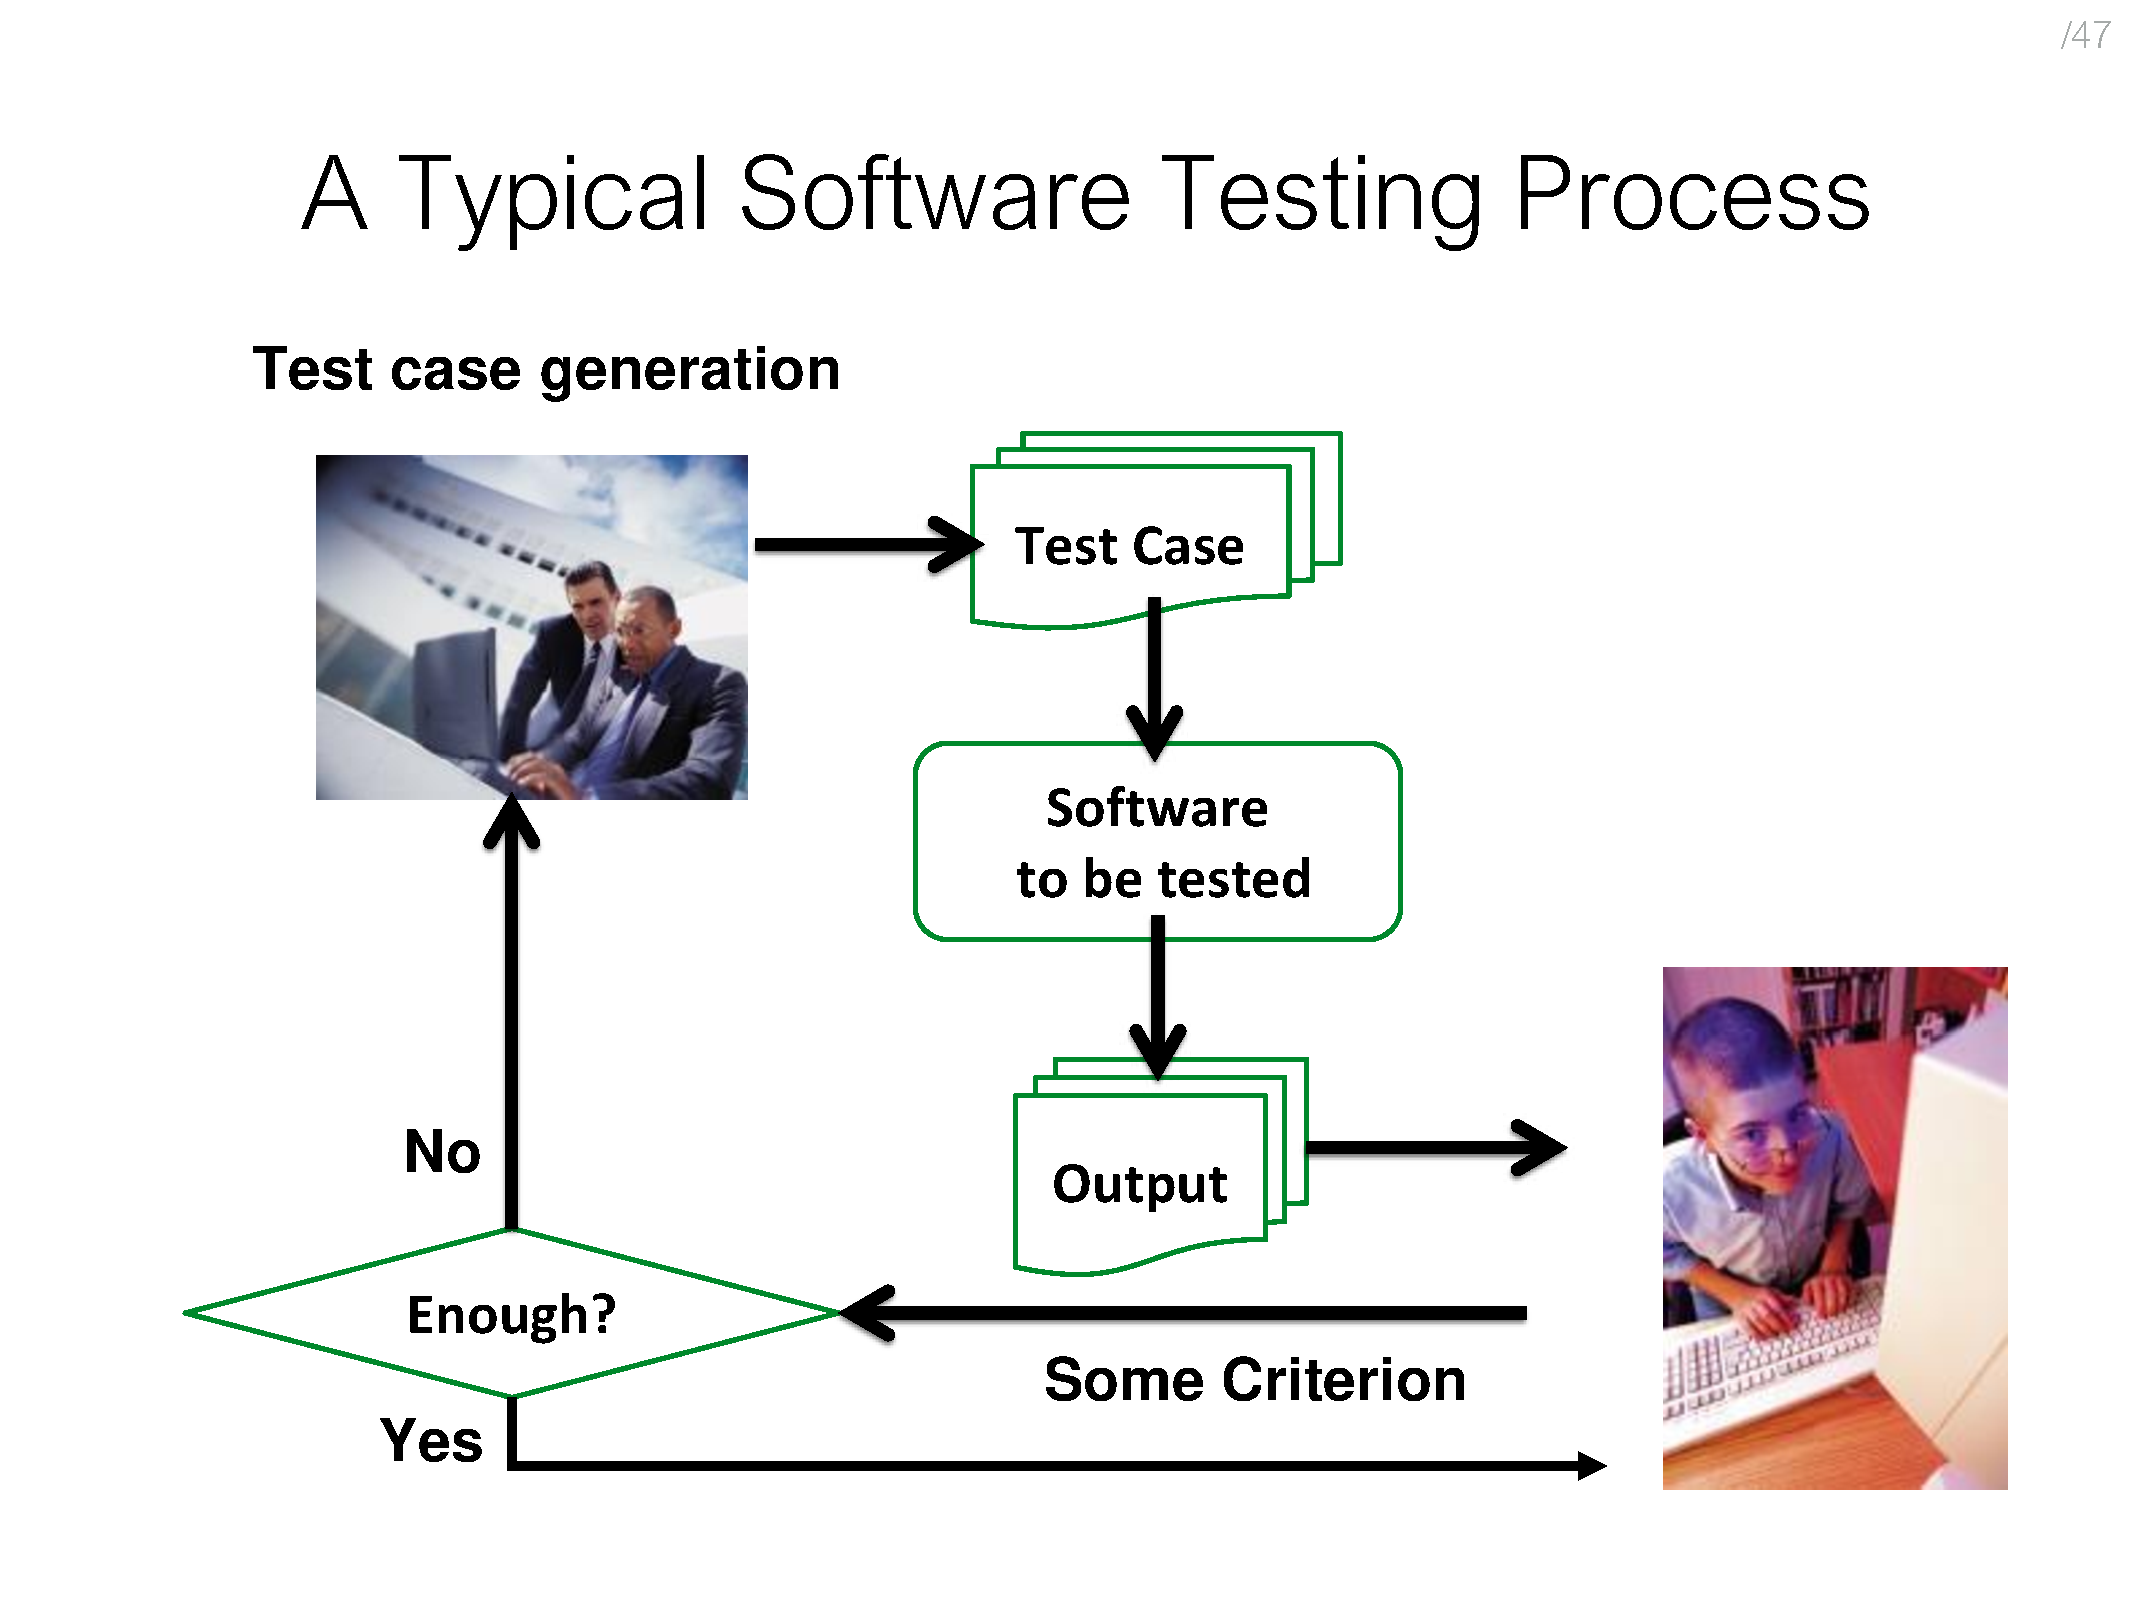
\includegraphics[width=\linewidth]{22.pdf}\\
        \textbf{Testing}: find inputs that cause failure of software, failure unknown, performed by testers\\
        \textbf{Debugging}: process of finding \& fixing fault given failure, failure is known, performed by devs\\
        \textbf{Black-Box/Functional Testing}: identify functions \& design test cases to check whether functions are correctly performed by software (formal \& informal specs)\\
        \textbf{Equivalence partitioning}: divide into partitions, select 1 test case from each partition, partitions must be disjointed (no input belongs to more than 1 partition) \& all partitions must cover entire input domain\\
        \textbf{Equivalence partitioning examples}: isEven then even \& odd, password min 8 \& max 12 characters then less than, valid, more than\\
        \textbf{\textbf{Boundary-Value analysis}}: partition input domain, identify boundaries, select test data (for range $[R_1,R_2]$ less than $R_1$, equal to $R_1$, between, equal to $R_2$, greater than $R_2$, for unordered sets select in \& not in, for equality select equal \& not equal, for sets, lists select empty \& not empty)\\
        \textbf{White box/structural testing}: generate test cases based on program structure, abstract program to control flow graph (node is sequence of statements, edge is transfers of control)\\
        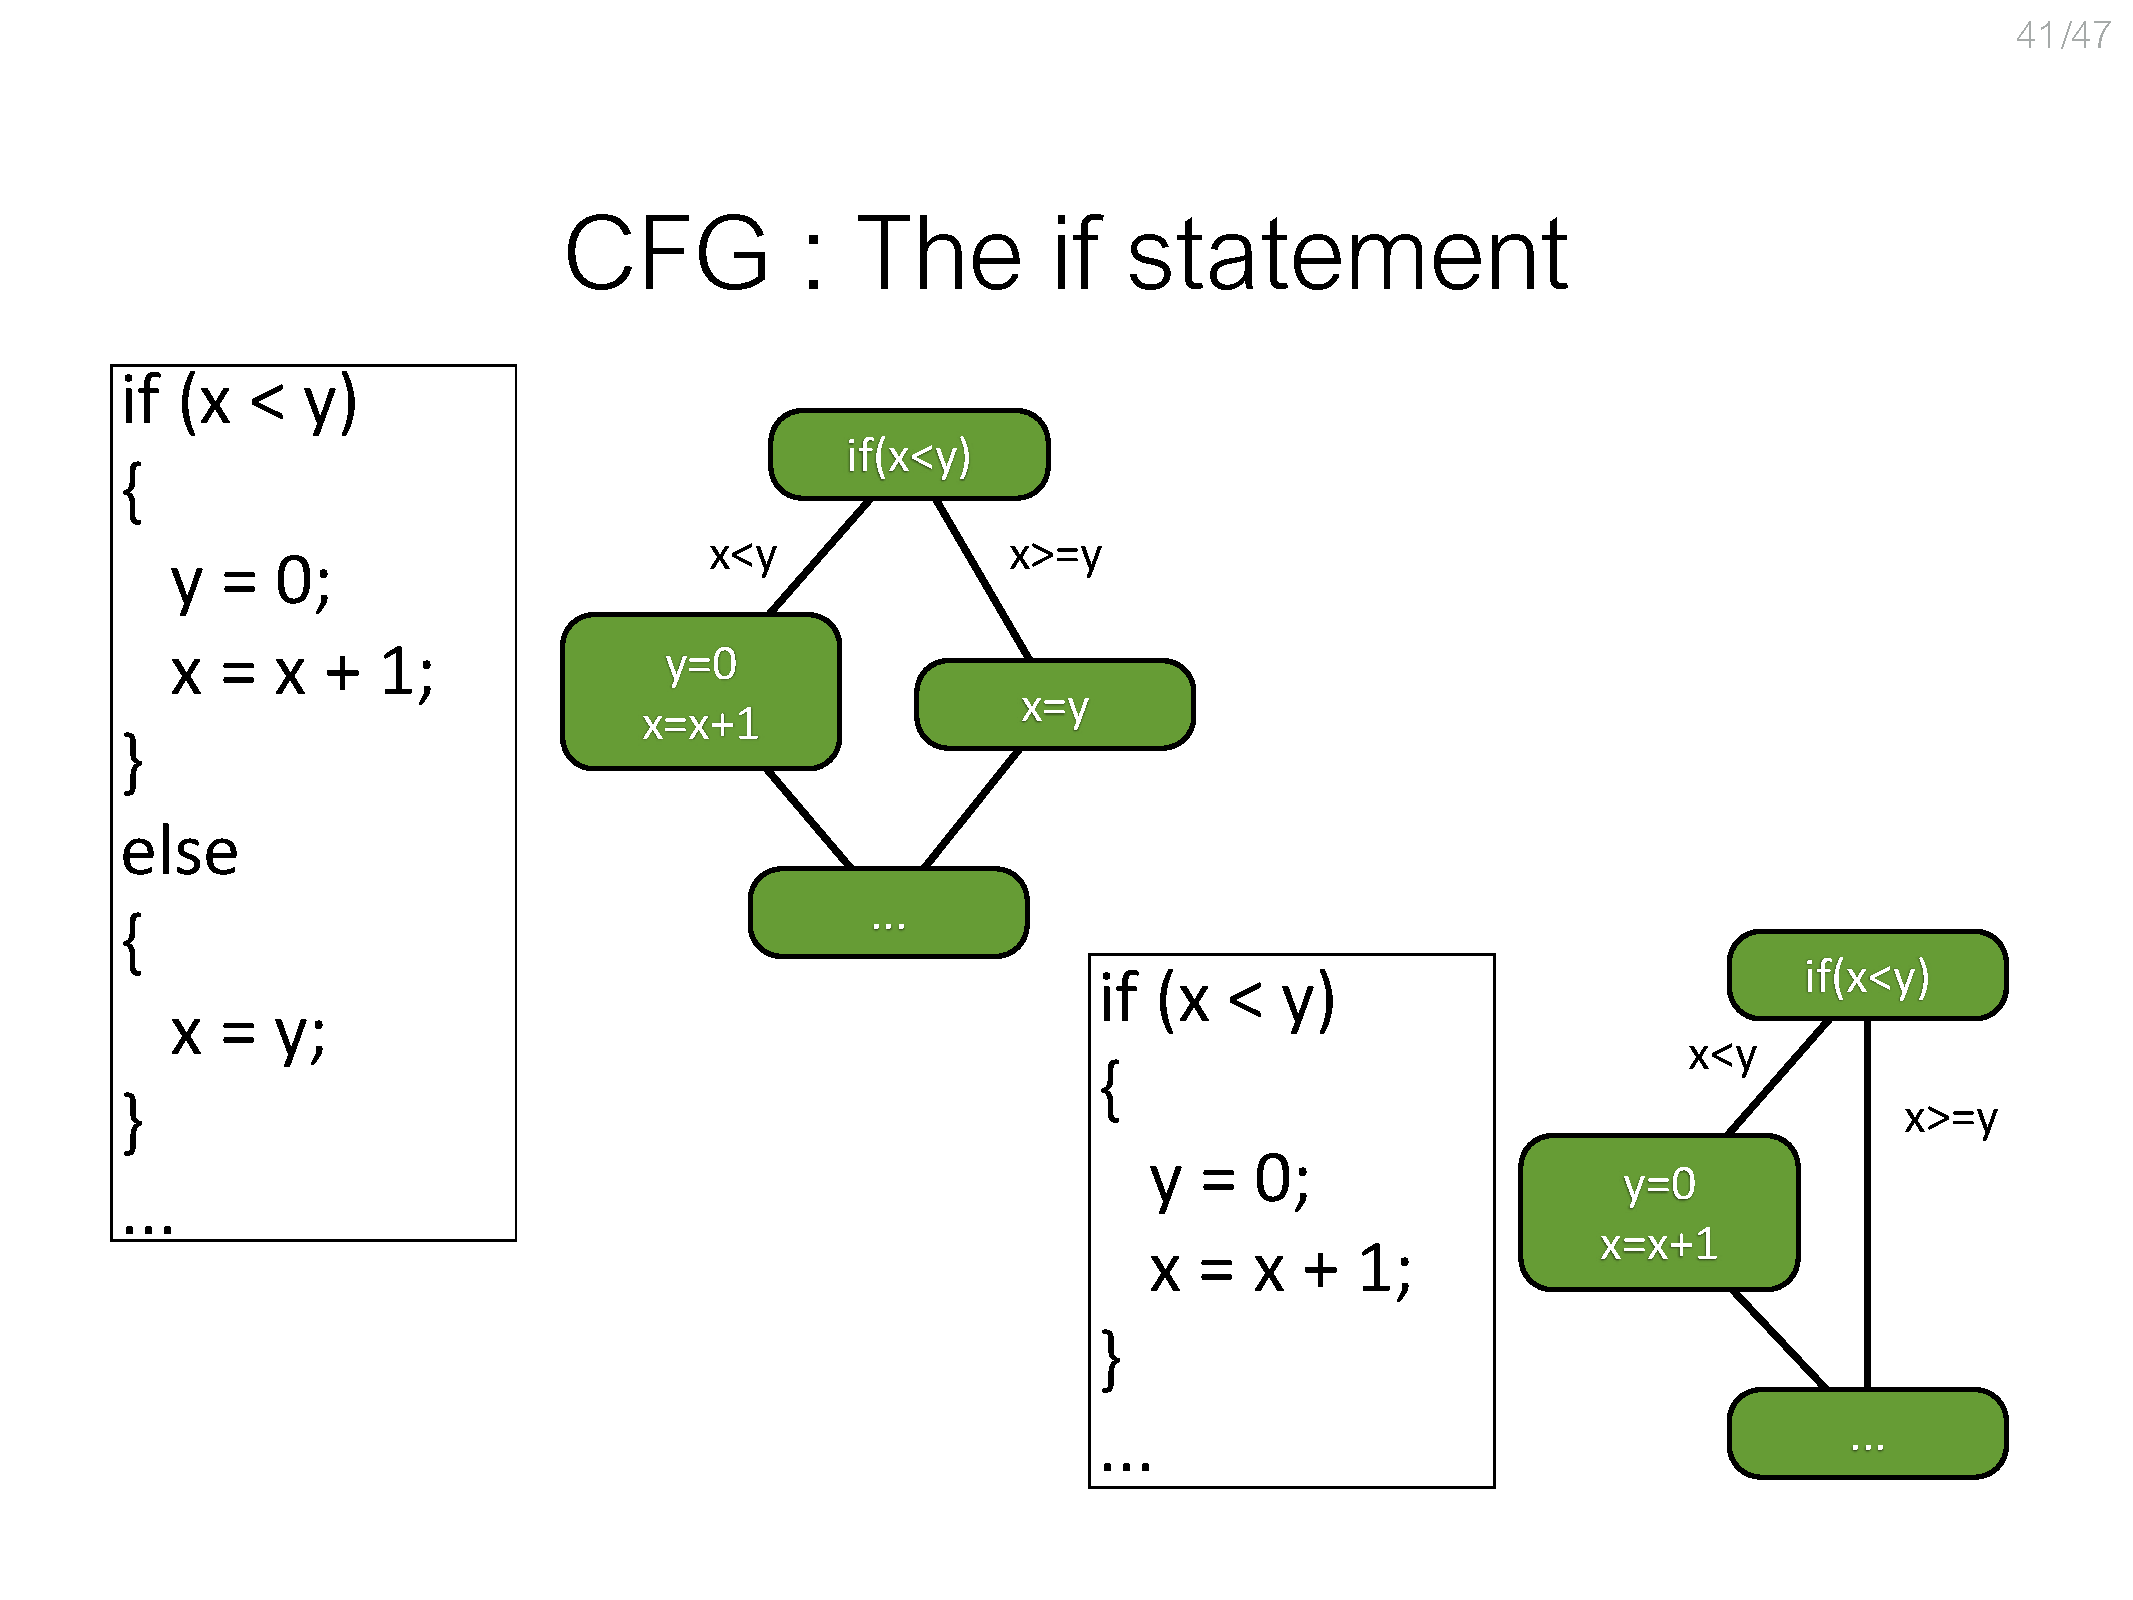
\includegraphics[width=\linewidth]{41.pdf}\\
        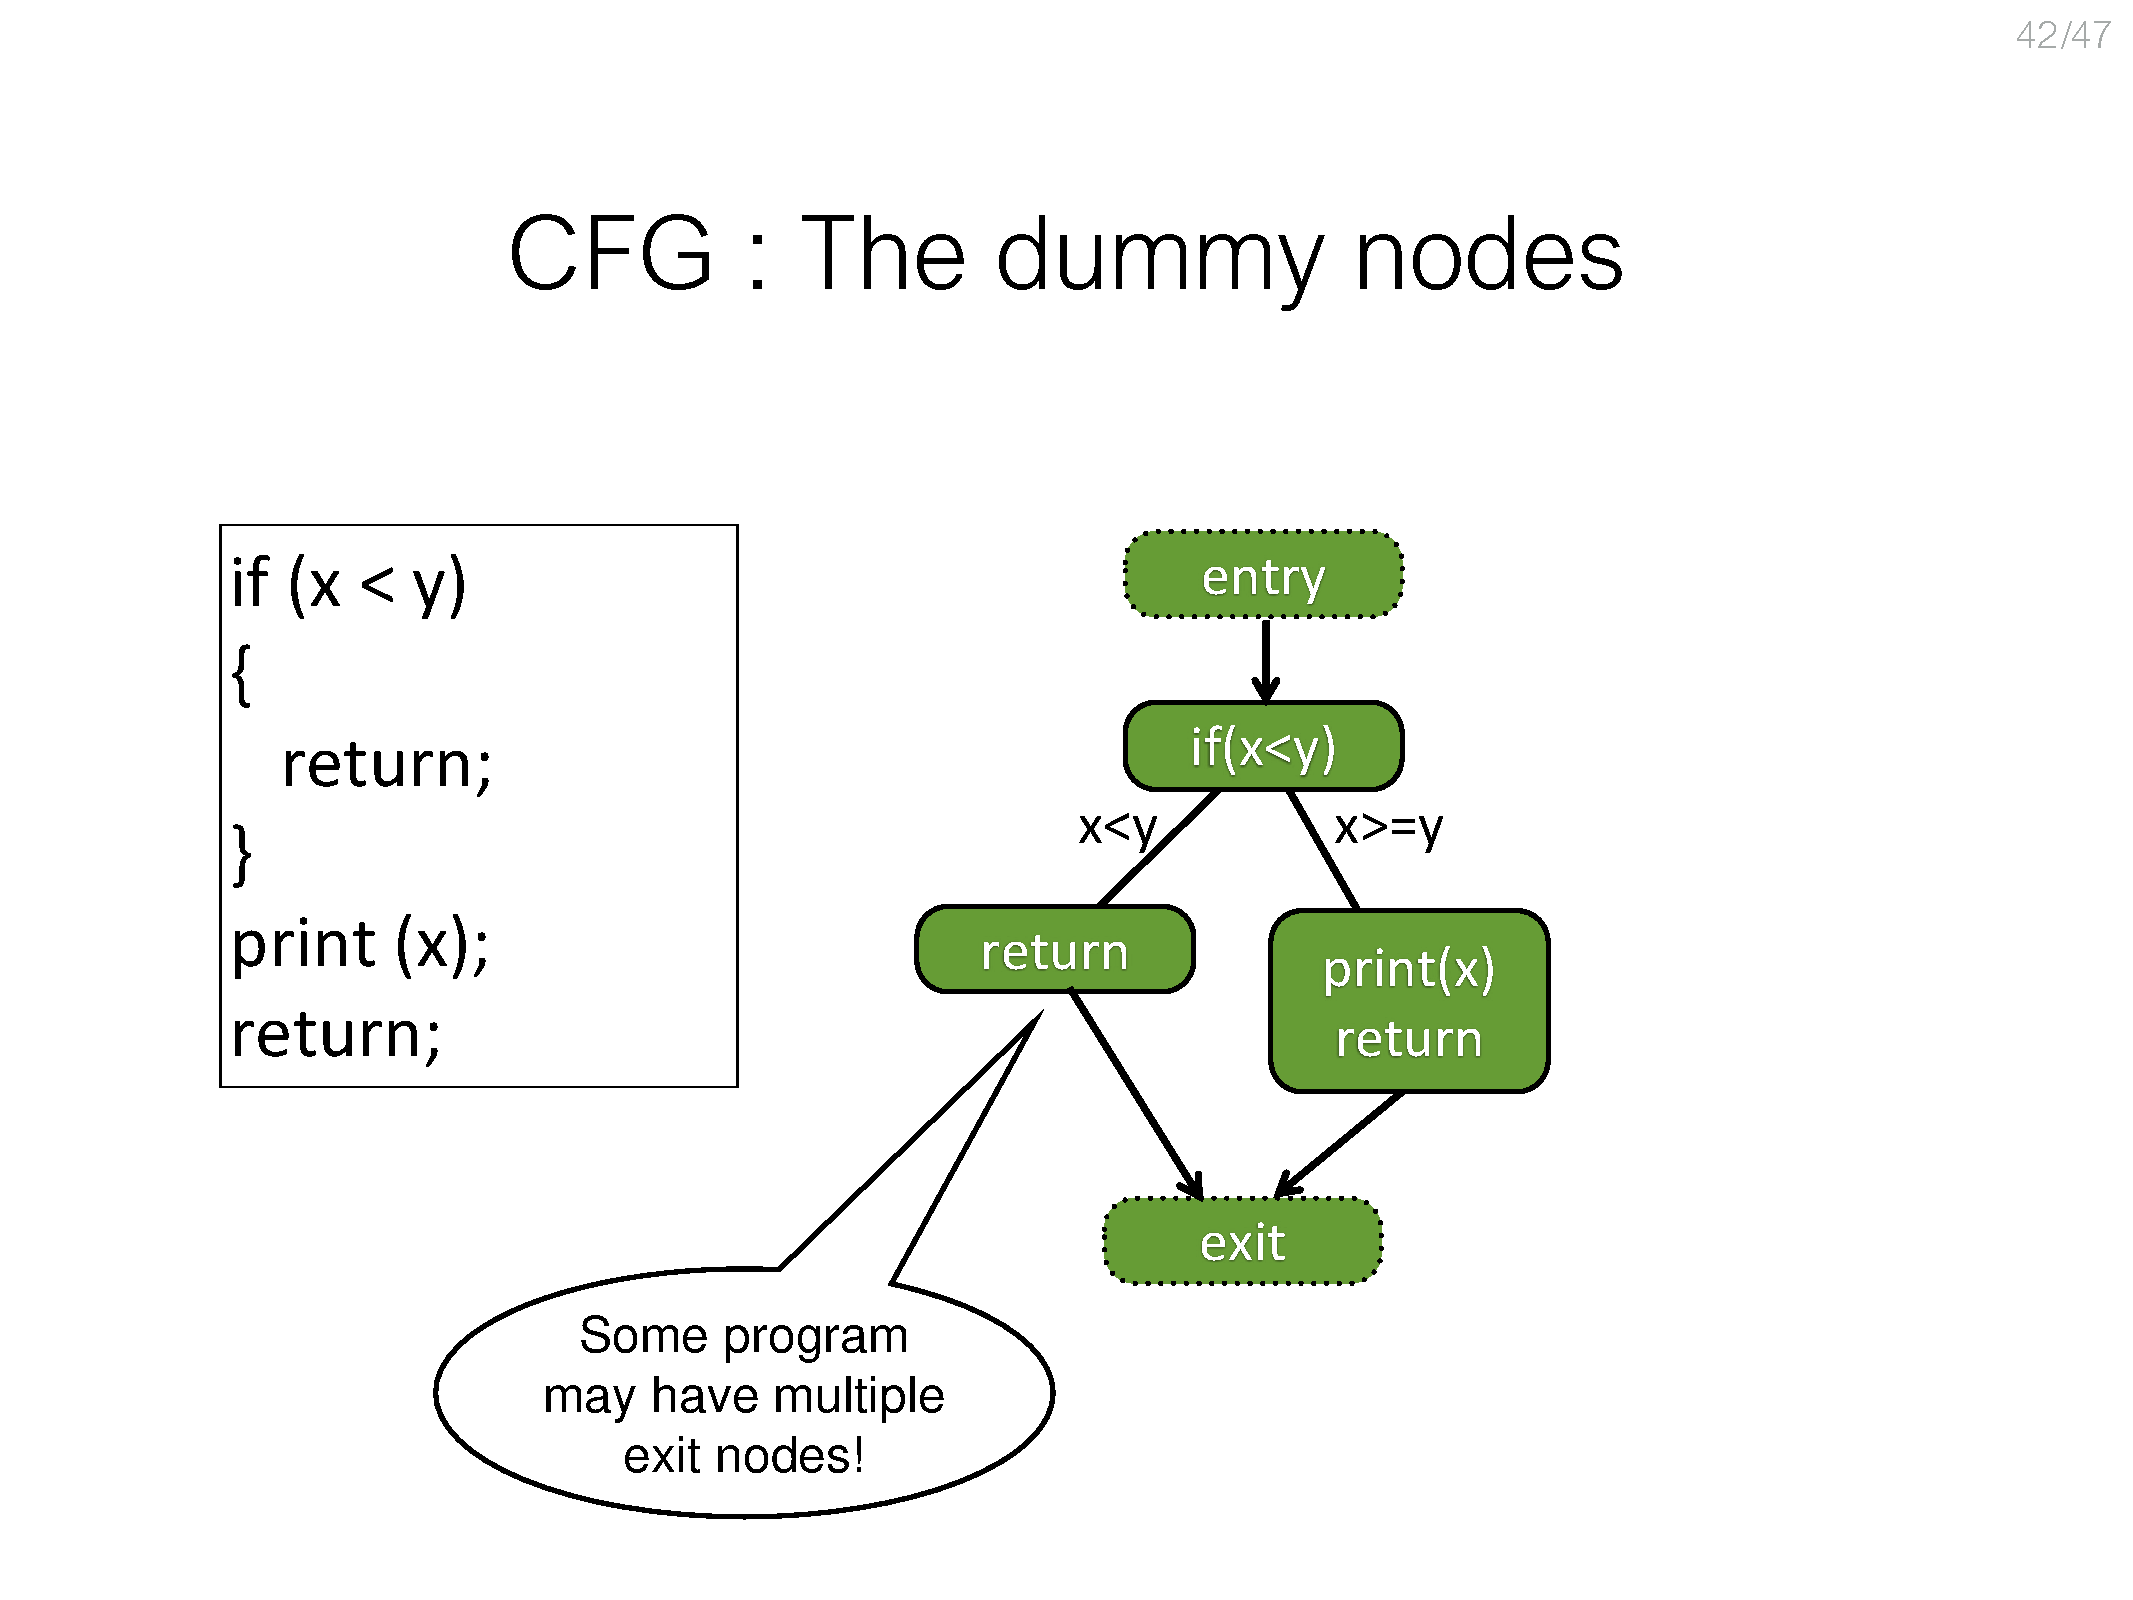
\includegraphics[width=\linewidth]{42.pdf}\\
        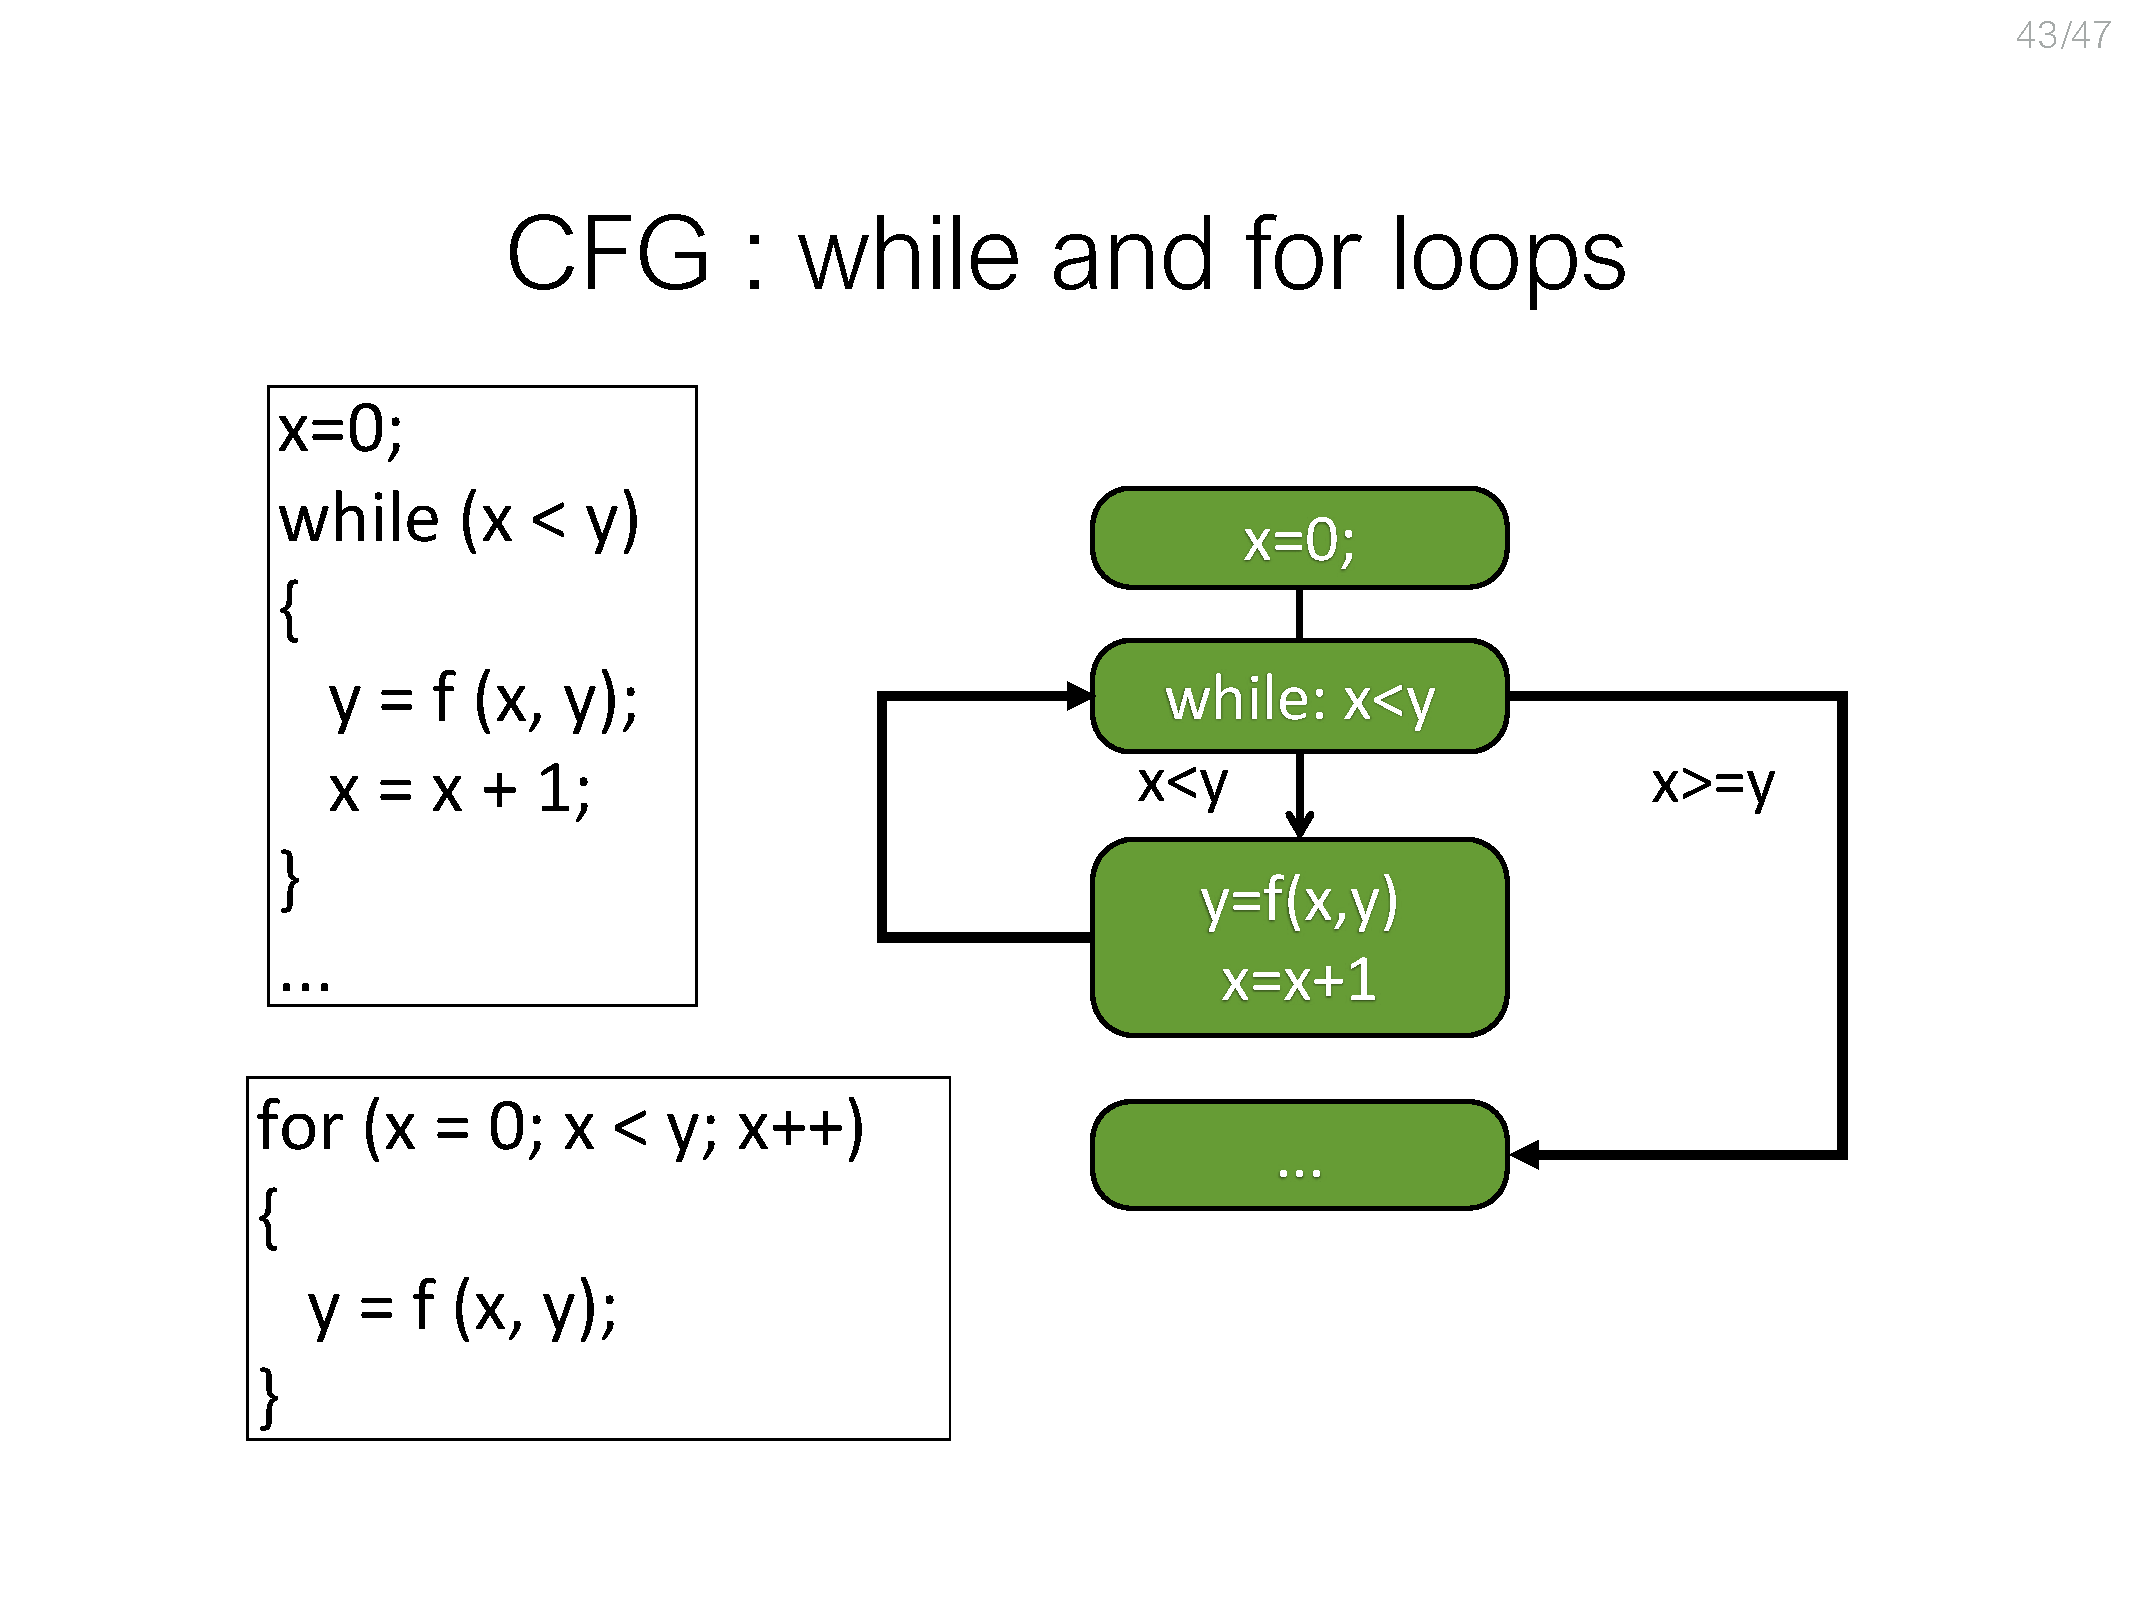
\includegraphics[width=\linewidth]{43.pdf}\\
        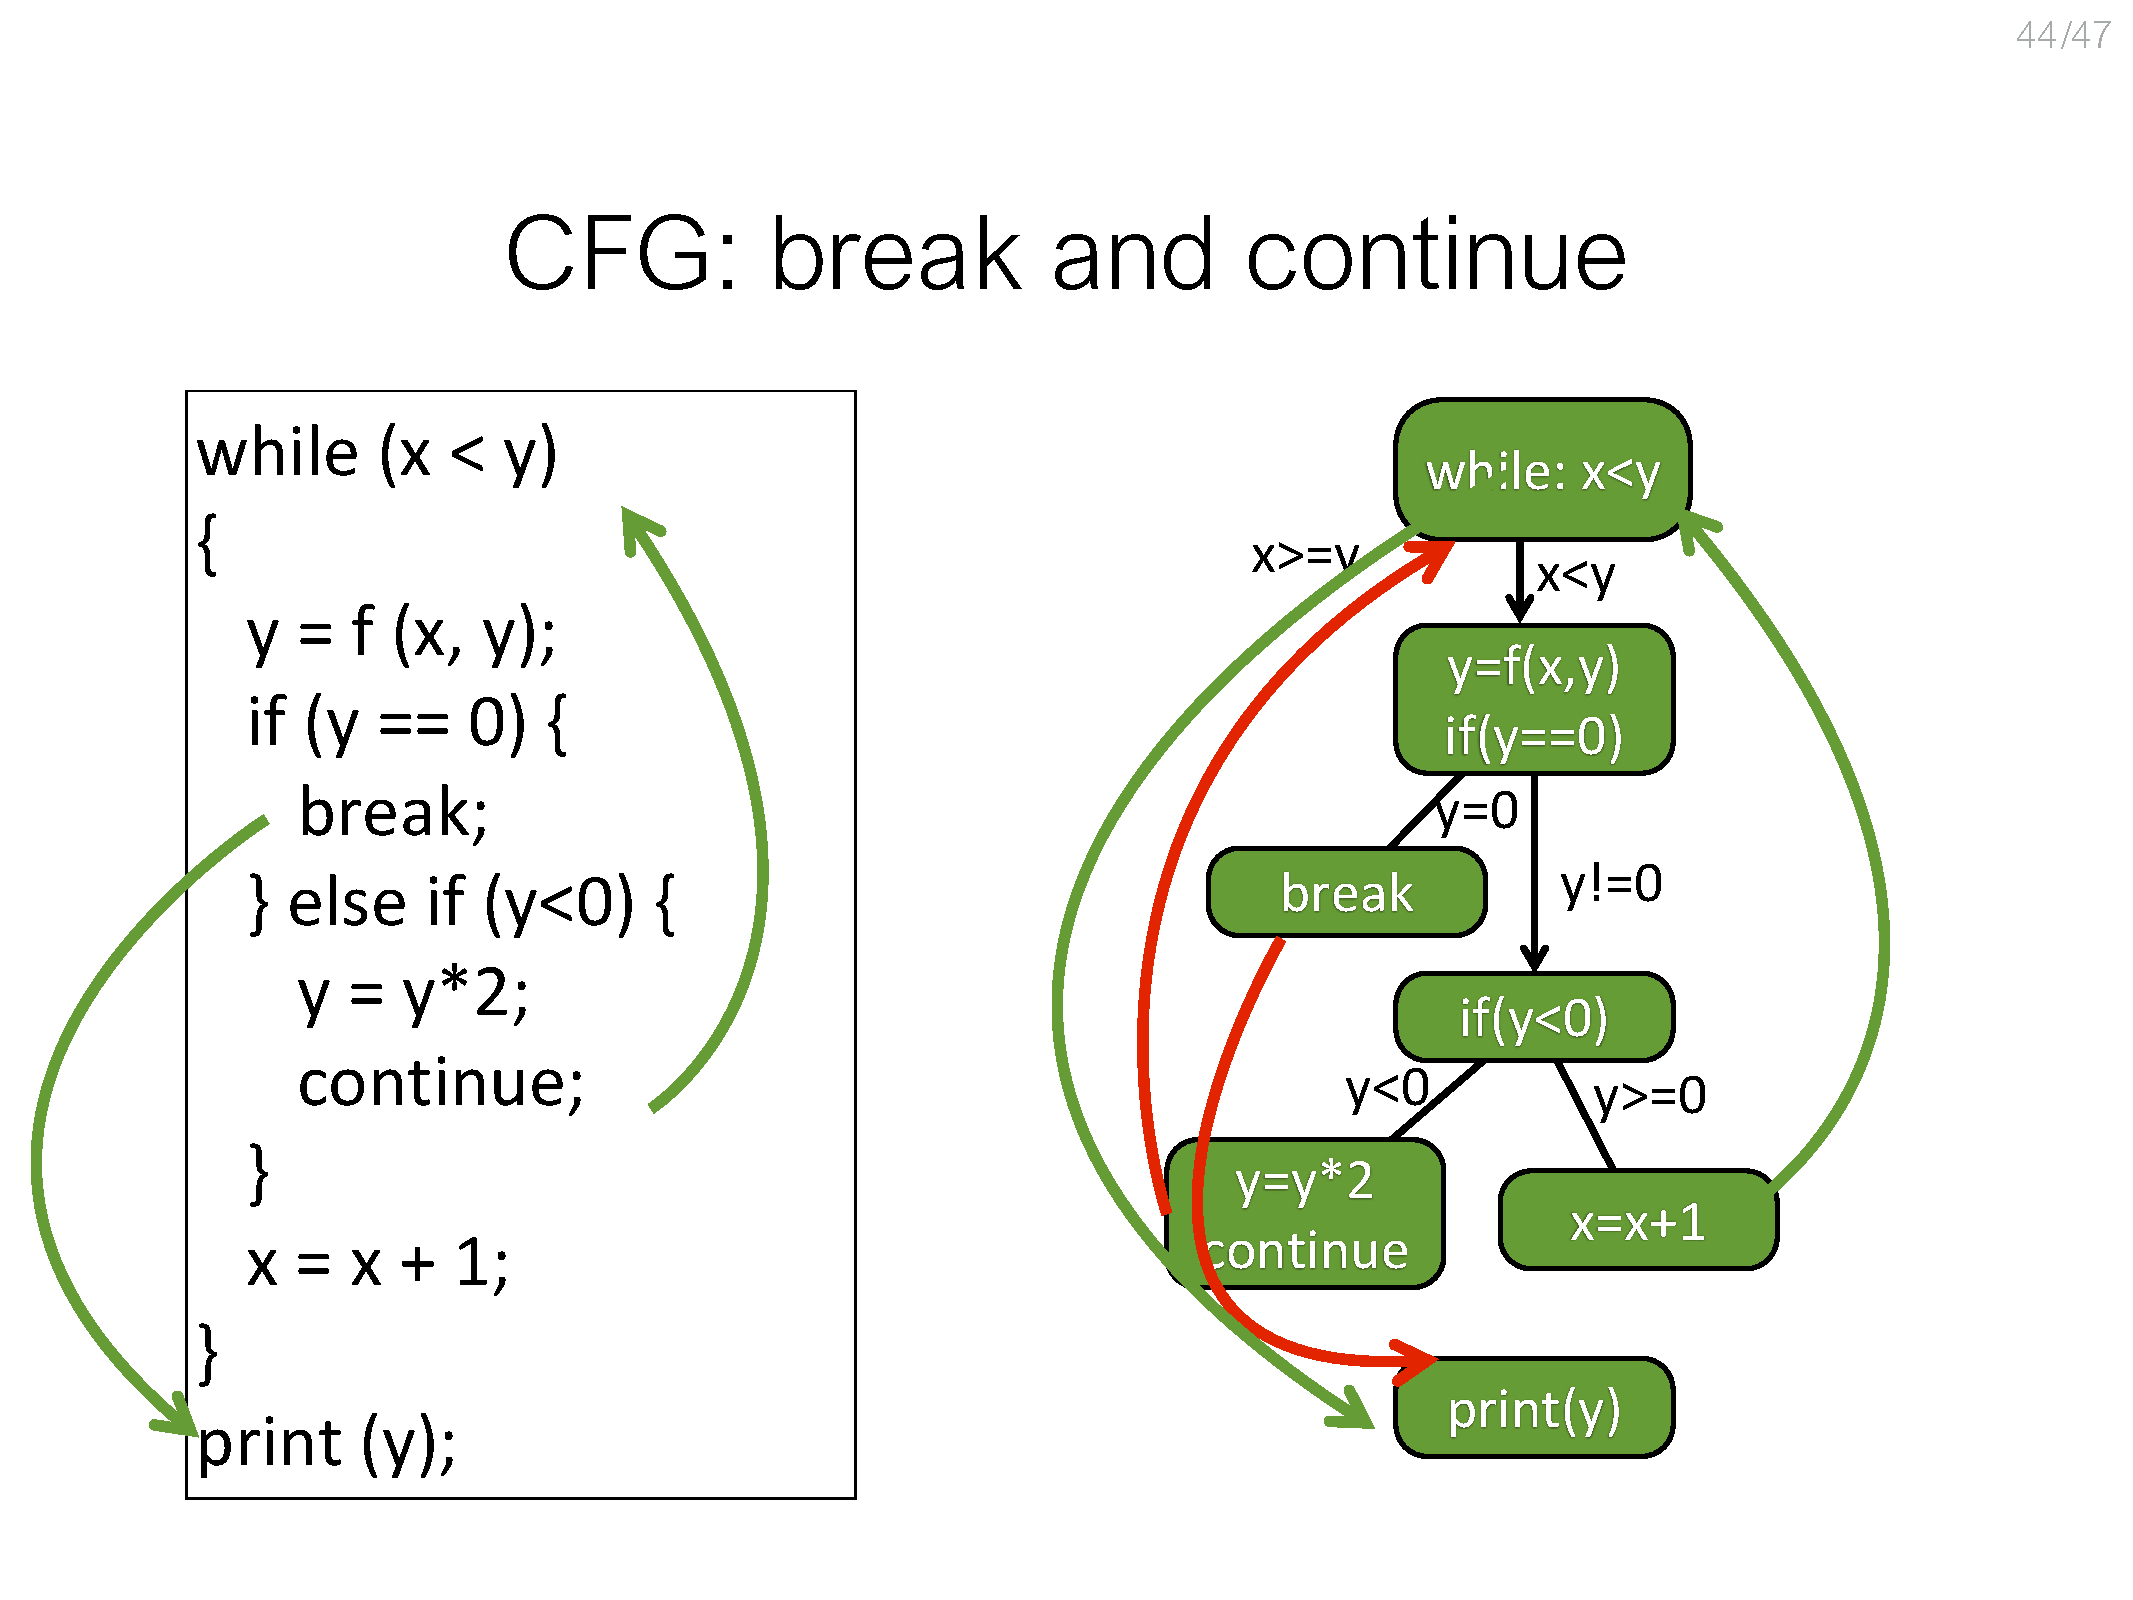
\includegraphics[width=\linewidth]{44.pdf}\\
        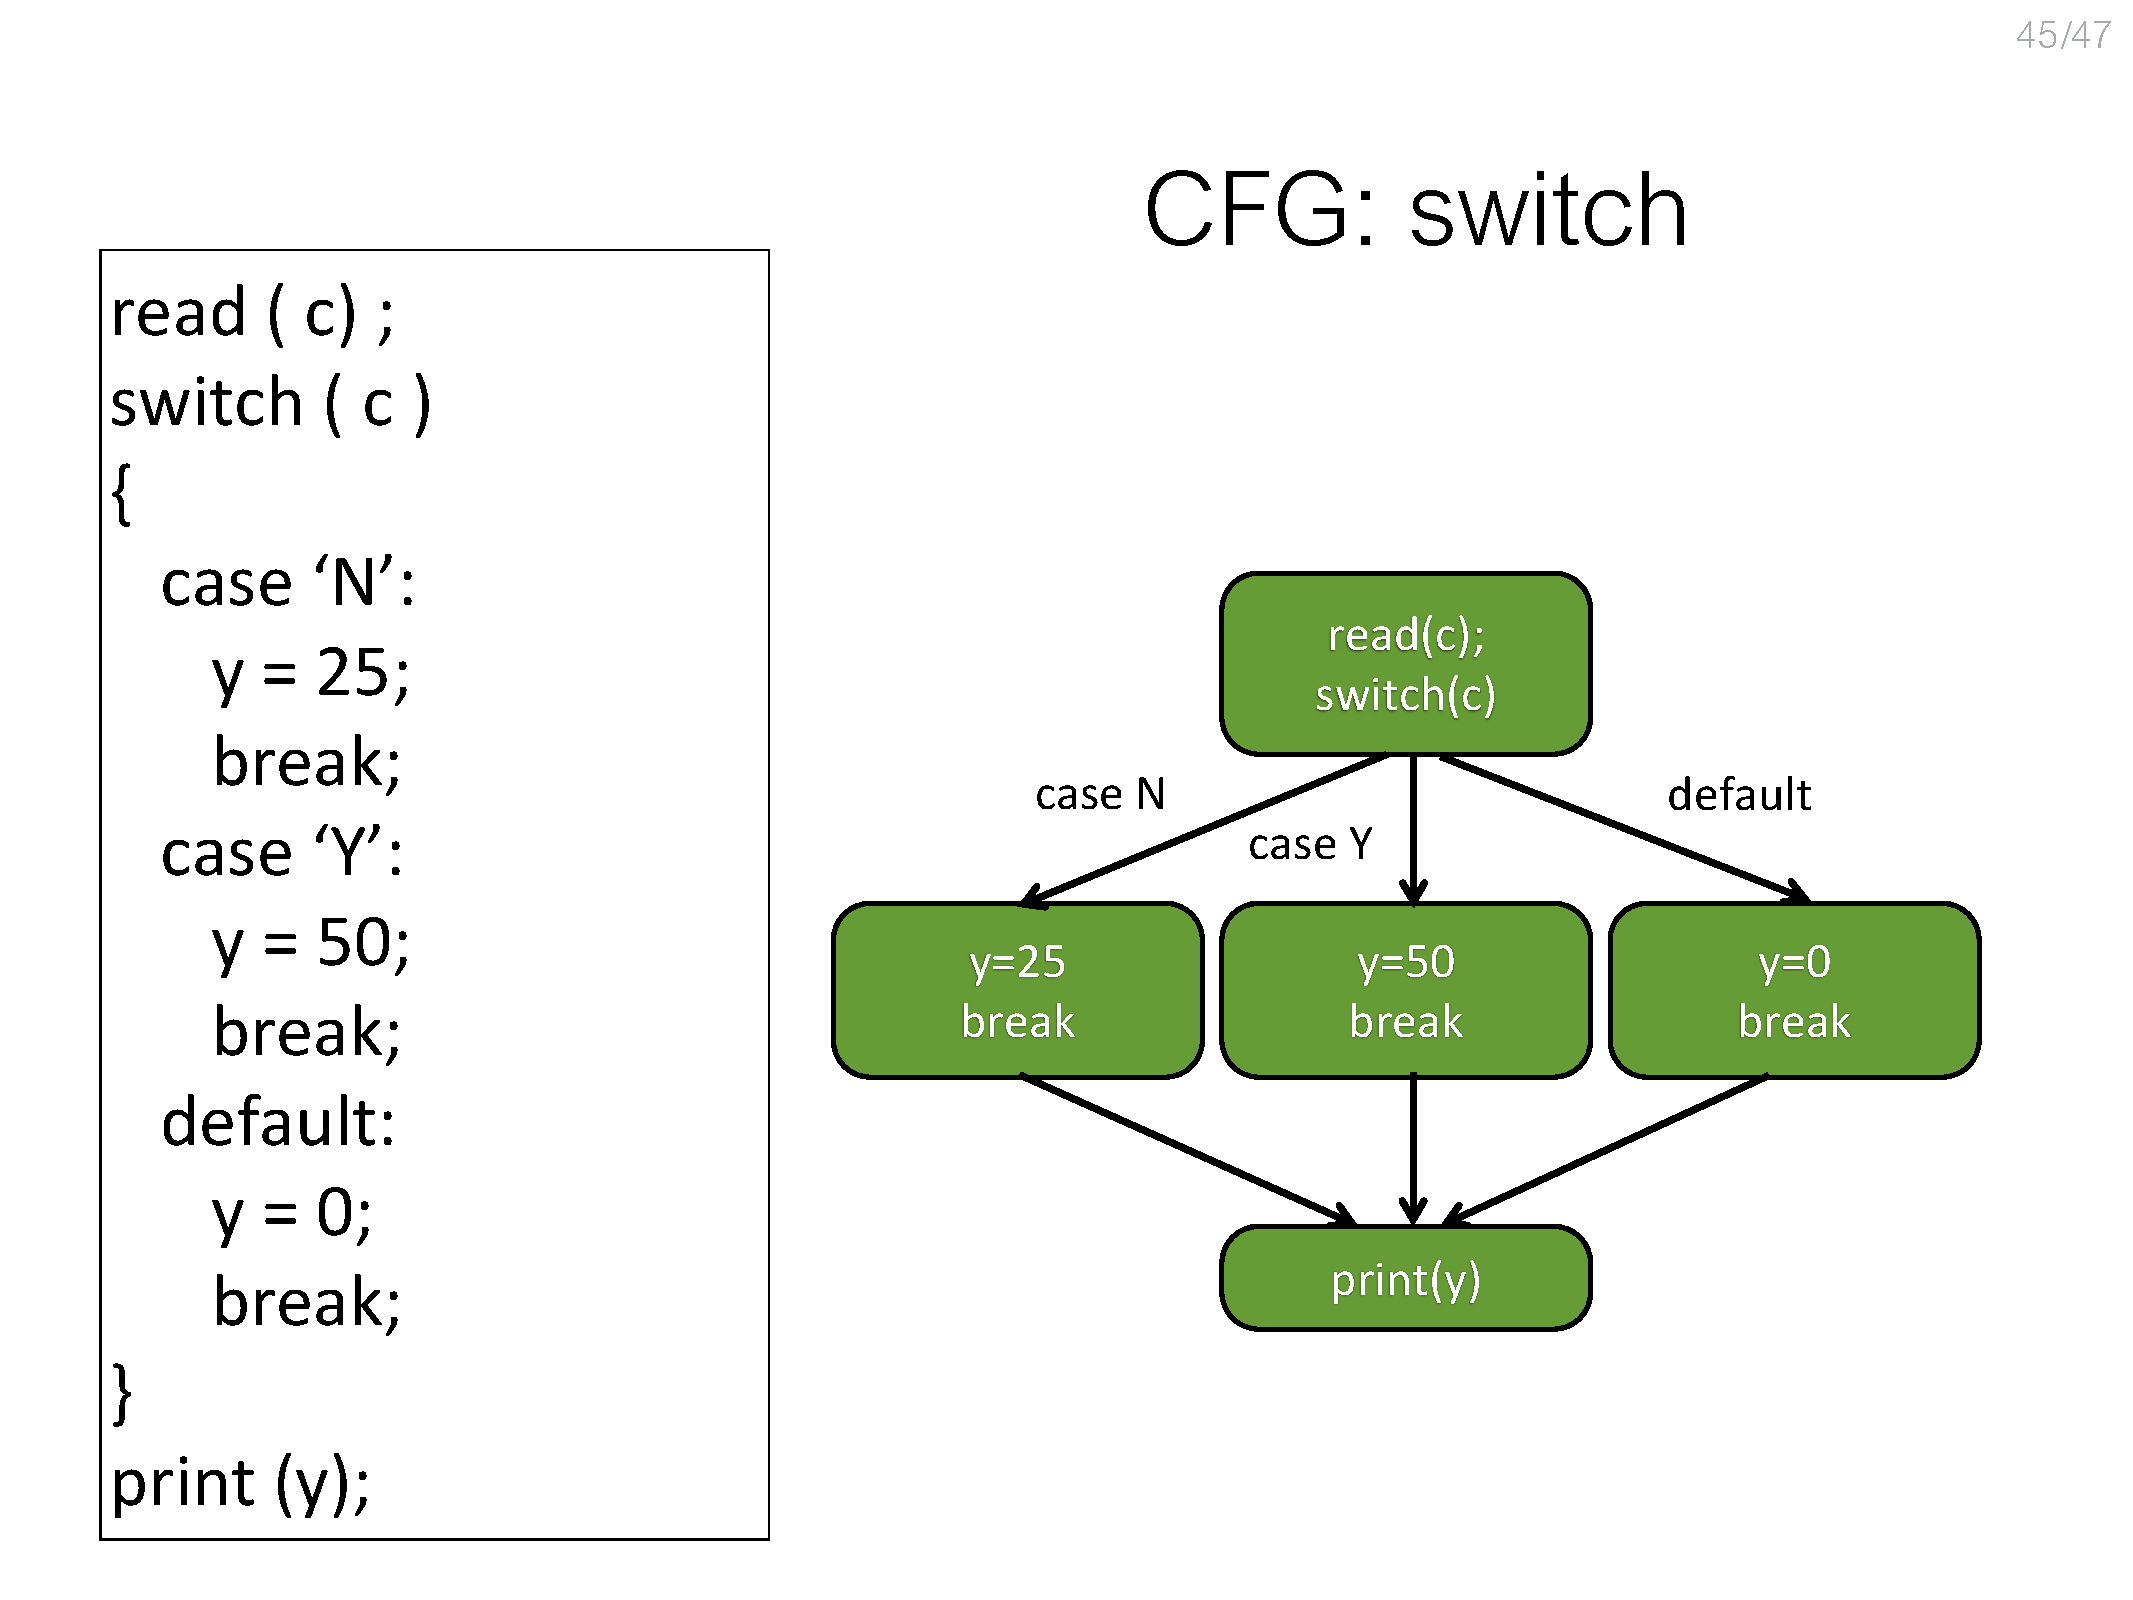
\includegraphics[width=\linewidth]{45.pdf}\\
        \textbf{Coverage types}: statement, branch, path (infinite if loop exists), strictly subsumes all beforehand\\
        \underline{\textbf{Week 2}}\\
        \textbf{Test oracle}: expected output of software for given input, part of test case\\
        \textbf{Test driver}: software framework that can load collection of test cases or test suite\\
        \textbf{Test suite}: collection of test cases\\
        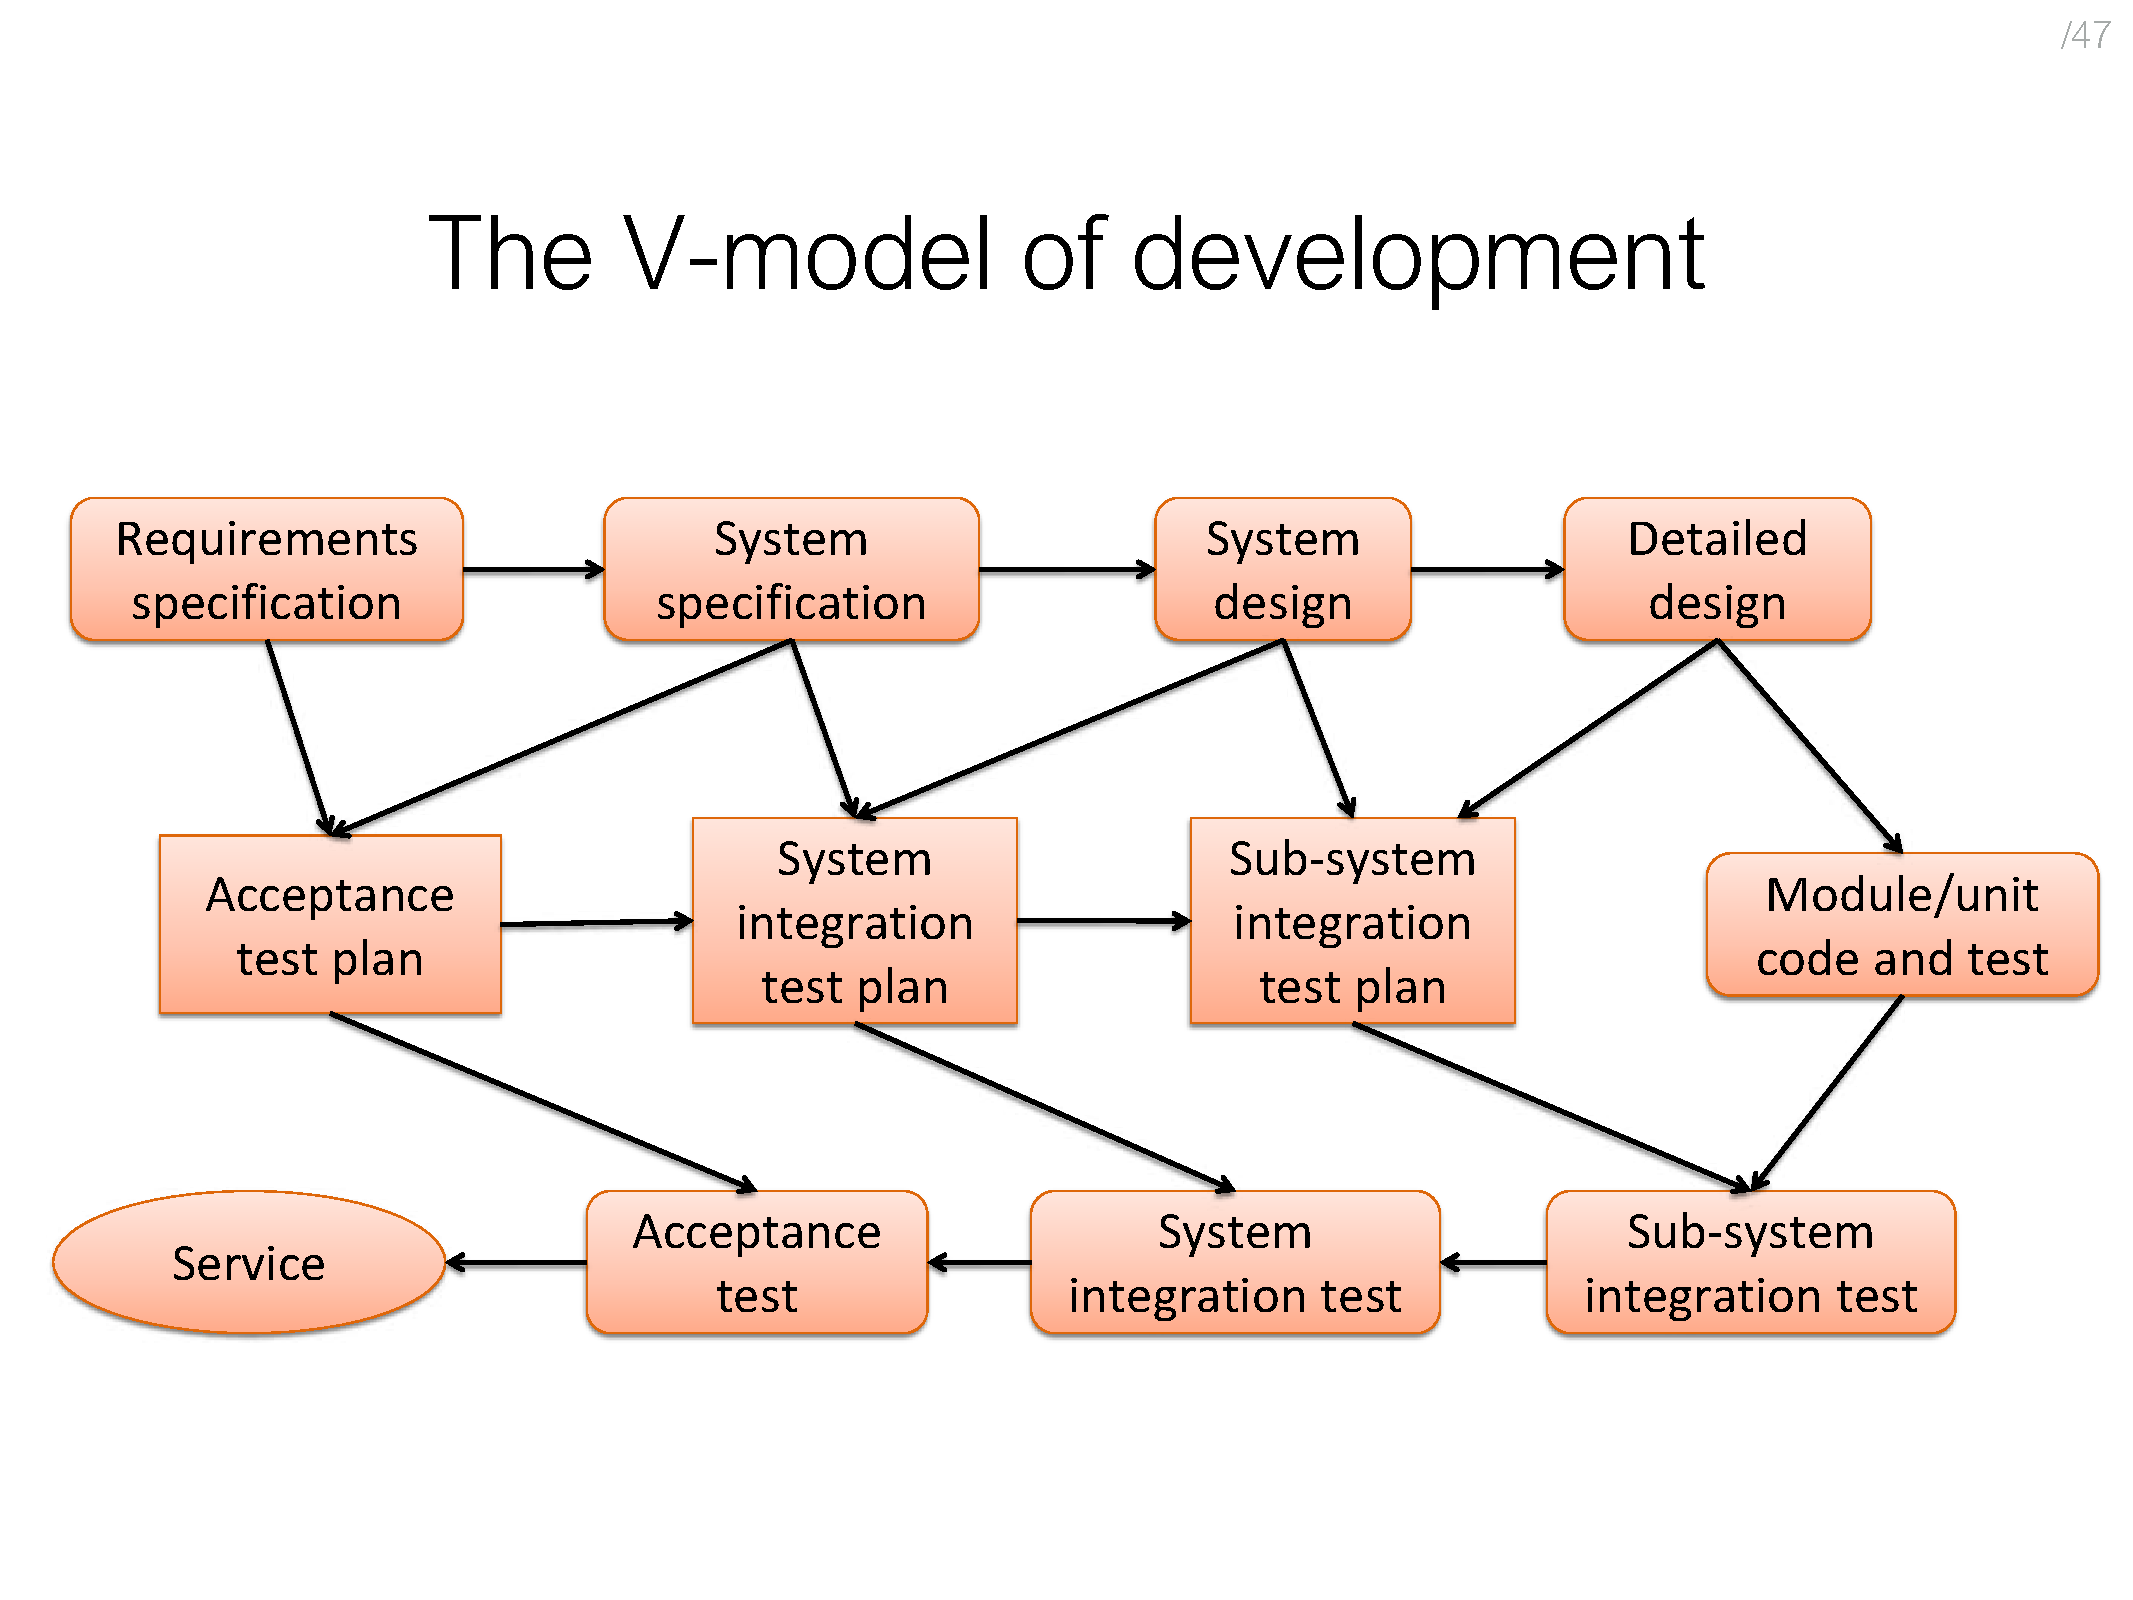
\includegraphics[width=\linewidth]{96.pdf}\\
        \textbf{Testing types}:\\
        \textit{Unit/Module}: test single module in isolated environment, use drivers \& stubs for isolation\\
        \textit{Integration}: test parts of system by combining modules, integrated collection of modules tested as group or partial system\\
        \textit{System}: test system as a whole after integration phase\\
        \textit{Acceptance}: test system as a whole to find out if it satisfies requirements specifications\\
        \textbf{Driver}: program that calls interface procedures of module being tested \& reports results, simulates module that calls module currently being tested, also provides access to global variables for module under test\\
        \textbf{Stub}: program that has same interface as module being used by module being tested but simpler, simulates module called by module being tested\\
        \textbf{Mock objects}: create object that mimics behaviour needed for testing\\
        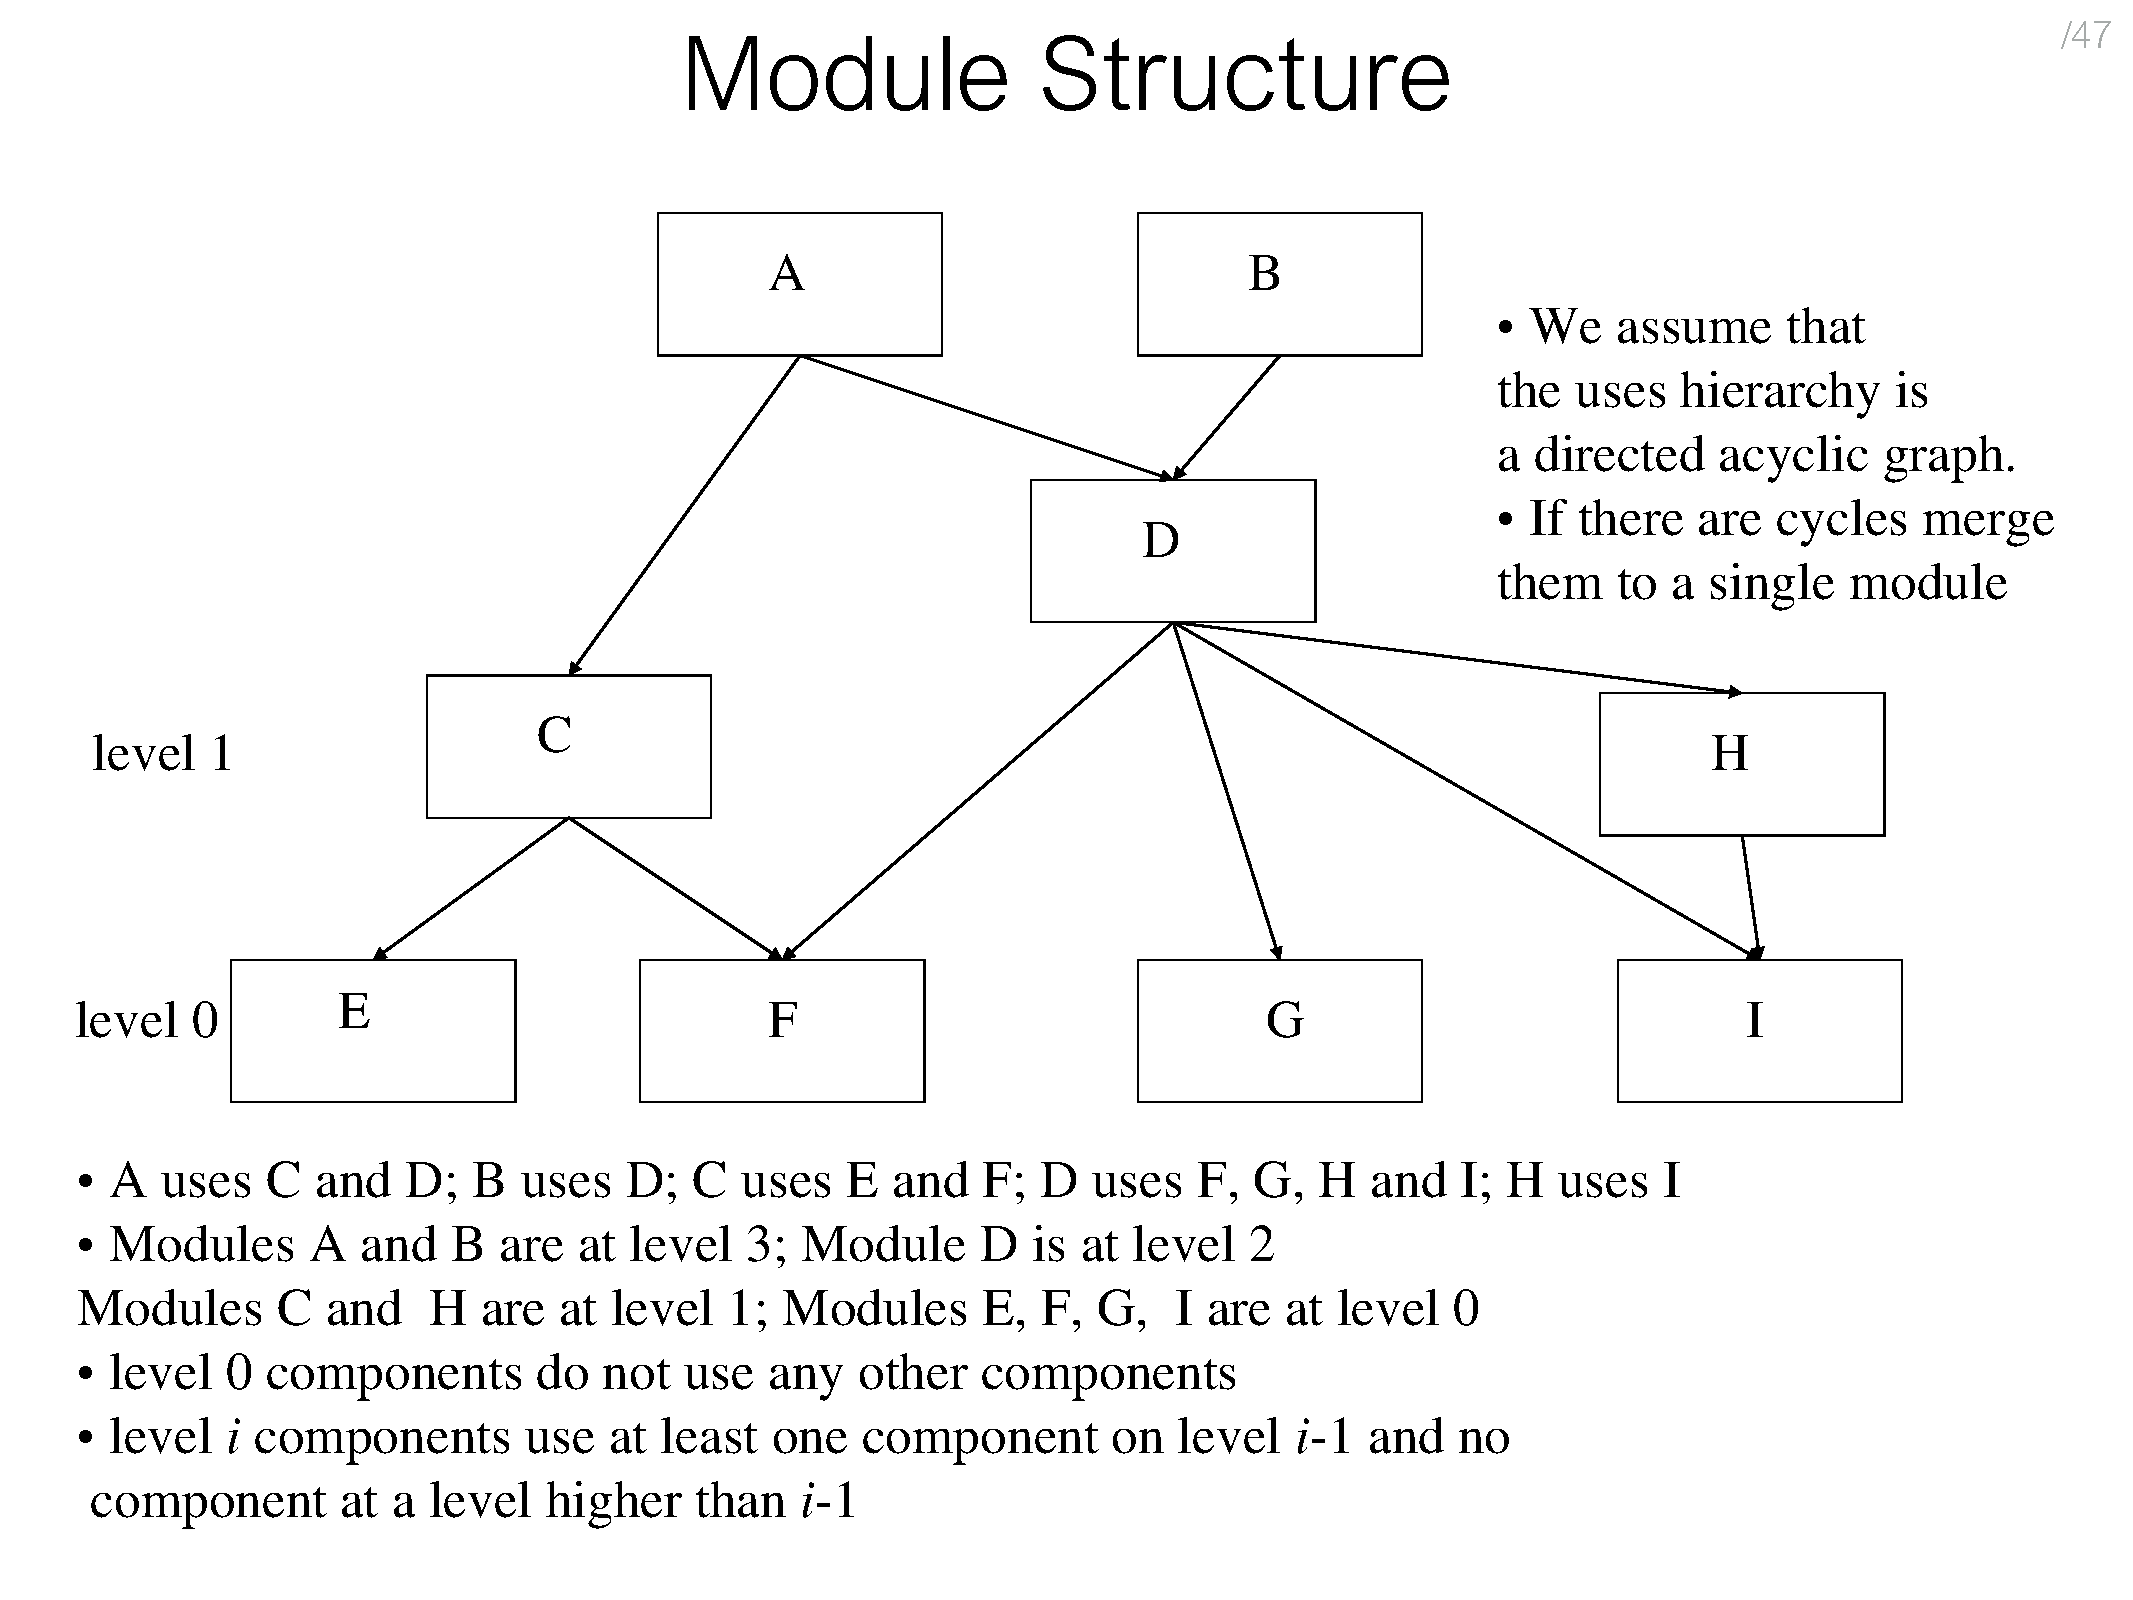
\includegraphics[width=\linewidth]{102.pdf}\\
        \textbf{Integration types}:\\
        \textit{Bottom-Up}: only terminal modules tested in isolation, requires drivers but not stubs (since lower levels are tested already)\\
        \textit{Top-down}: modules tested in isolation are modules at highest level, requires stubs but not drivers\\
        \textit{Sandwich}: begin both bottom-up \& top-down, meet at predetermined point in middle\\
        \textit{Big bang}: every module unit tested, then integrate all at once, no driver or stub needed but may be hard to isolate bugs\\
        \textbf{System/Acceptance testing}: can construct test case based on requirements specifications, main purpose is to assure that system meets requirements, alpha testing performed within development organisation, beta testing performed by select group of friendly customers\\
        \underline{\textbf{Week 3}}\\
        \textbf{Basis Path Testing}: between branch \& path coverage, fulfills branch testing \& tests all independent paths that could be used to construct any arbitrary path through computer program\\
        \textbf{Independent path}: includes some vertices/edges not covered in other path\\
        \textbf{Cyclomatic complexity}: $e-n+2p$, $e$ is edges, $n$ is nodes, $p$ is number of connected components, or $1+d$, $d$ is loops or decision points, upper bound on number of test cases to guarantee coverage of all statements\\
        \textbf{Decision Coverage}: executing true/false of decision\\
        \textbf{Condition Coverage}: executing true/false of each condition\\
        \textbf{Condition/Decision Coverage}: DC \& CC, better than either\\
        \textbf{Multiple Condition Coverage}: whether every possible combination of boolean sub-expressions occurs, test cases are truth table, $2^n$ test cases for $n$ conditions\\
        \textbf{Modified C/DC}: for each basic condition $C$, 2 test cases, values of all evaluated conditions except $C$ are the same, compound decision as a whle evaluates to true for 1 \& false for the other, subsumed by MCC \& subsumes CC, DC, C/DC, stronger than statement \& branch\\
        \textbf{MC/DC coverage}: each entry \& exit point invoked, each decision takes every possible outcome, each condition in a decision takes every possible outcome, each condition in decision is shown to independenly affect outcome of decision, independence of condition is shown by proving that only one condition changes at a time\\
        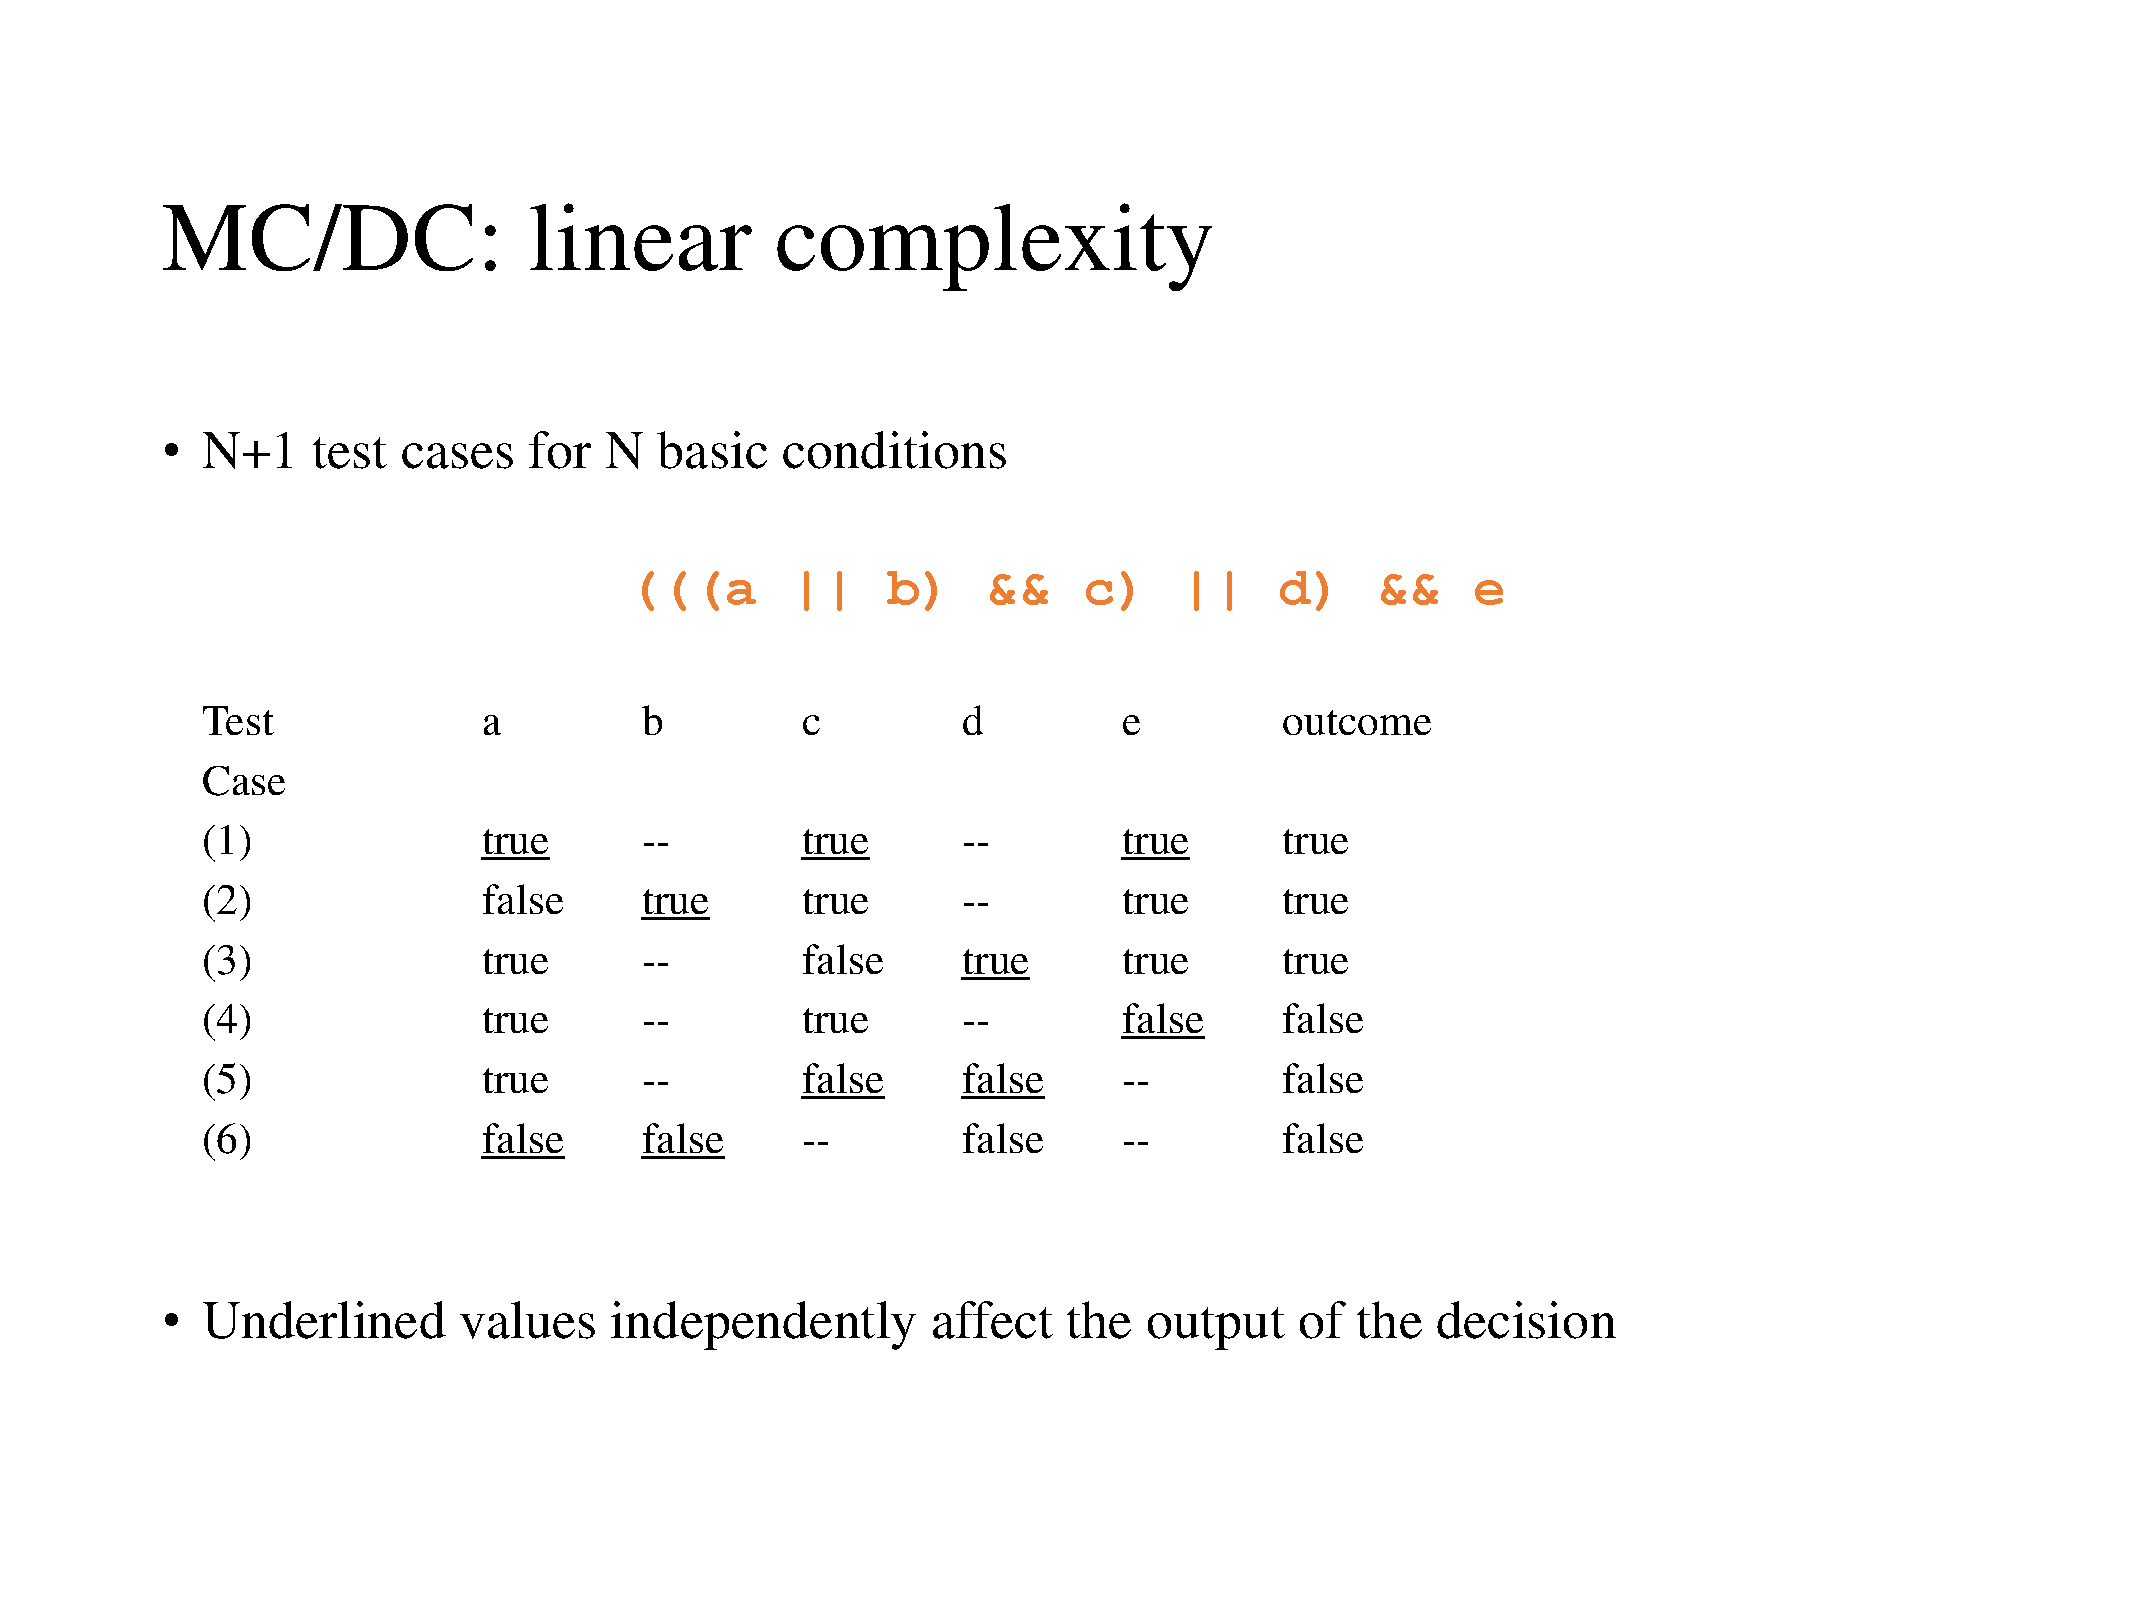
\includegraphics[width=\linewidth]{148.pdf}\\
        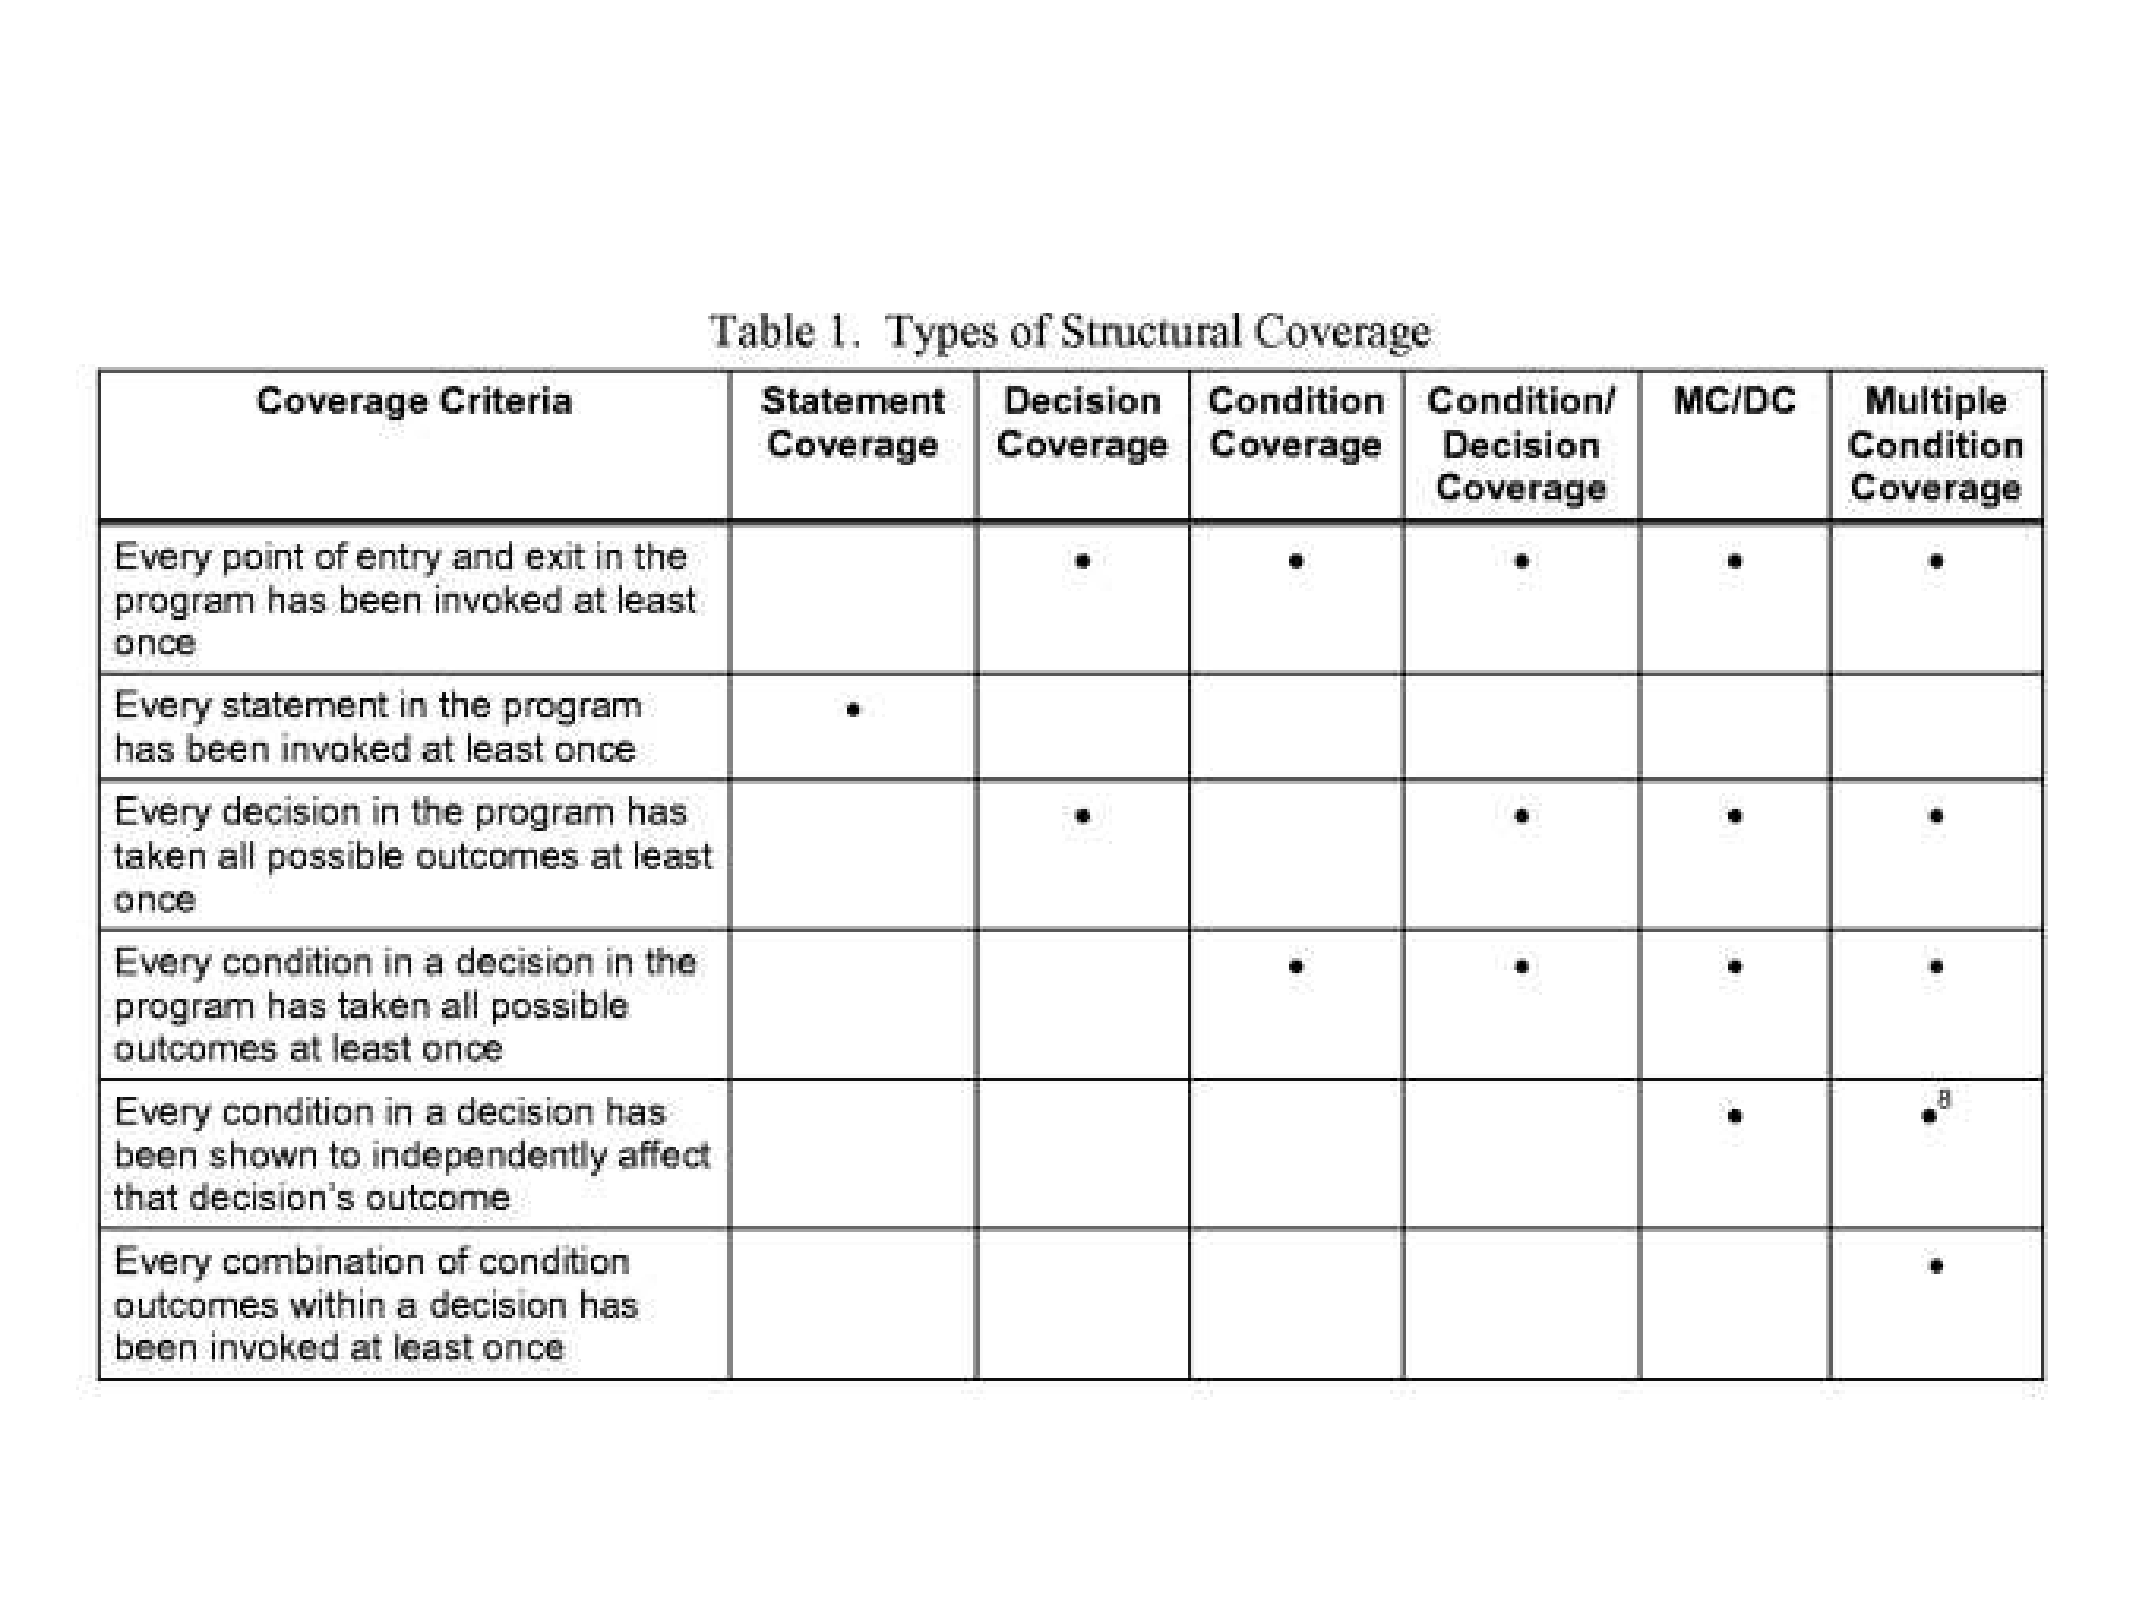
\includegraphics[width=\linewidth]{152.pdf}\\
        \underline{\textbf{Week 4}}\\
        \textbf{Dataflow Coverage}: considers how data gets accessed \& modified in system \& how it can get corrupted\\
        \textbf{Common access-related bugs}: using undefined/uninitializsed variable, deallocating/reinitialising variable before constructed/initialised/used, deleting collection object leaving members unaccessible\\
        \textbf{Variable definition}: defined whenever value modified (LHS of assignment, input statement, call-by-reference)\\
        \textbf{Variable use}: used whenever value read (RHS of assignment, call-by-value, branch statement predicate)\\
        \textbf{p-use}: use in predicate of branch statement\\
        \textbf{c-use}: any other use\\
        \textbf{Use \& redefine in single statement}: both sides of assignment, call-by-reference\\
        \textbf{du-pair}: with respect to variable $v$ is a pair $(d,u)$ such that $d$ is a node defining $v$, $u$ is a node/edge using $v$ (if p-use $u$ is outgoing edge of predicate), there is a def-clear path with respect to $v$ from $d$ to $u$\\
        \textbf{Definition clear}: with respect to variable $v$ if no variable re-definition of $v$ on path\\
        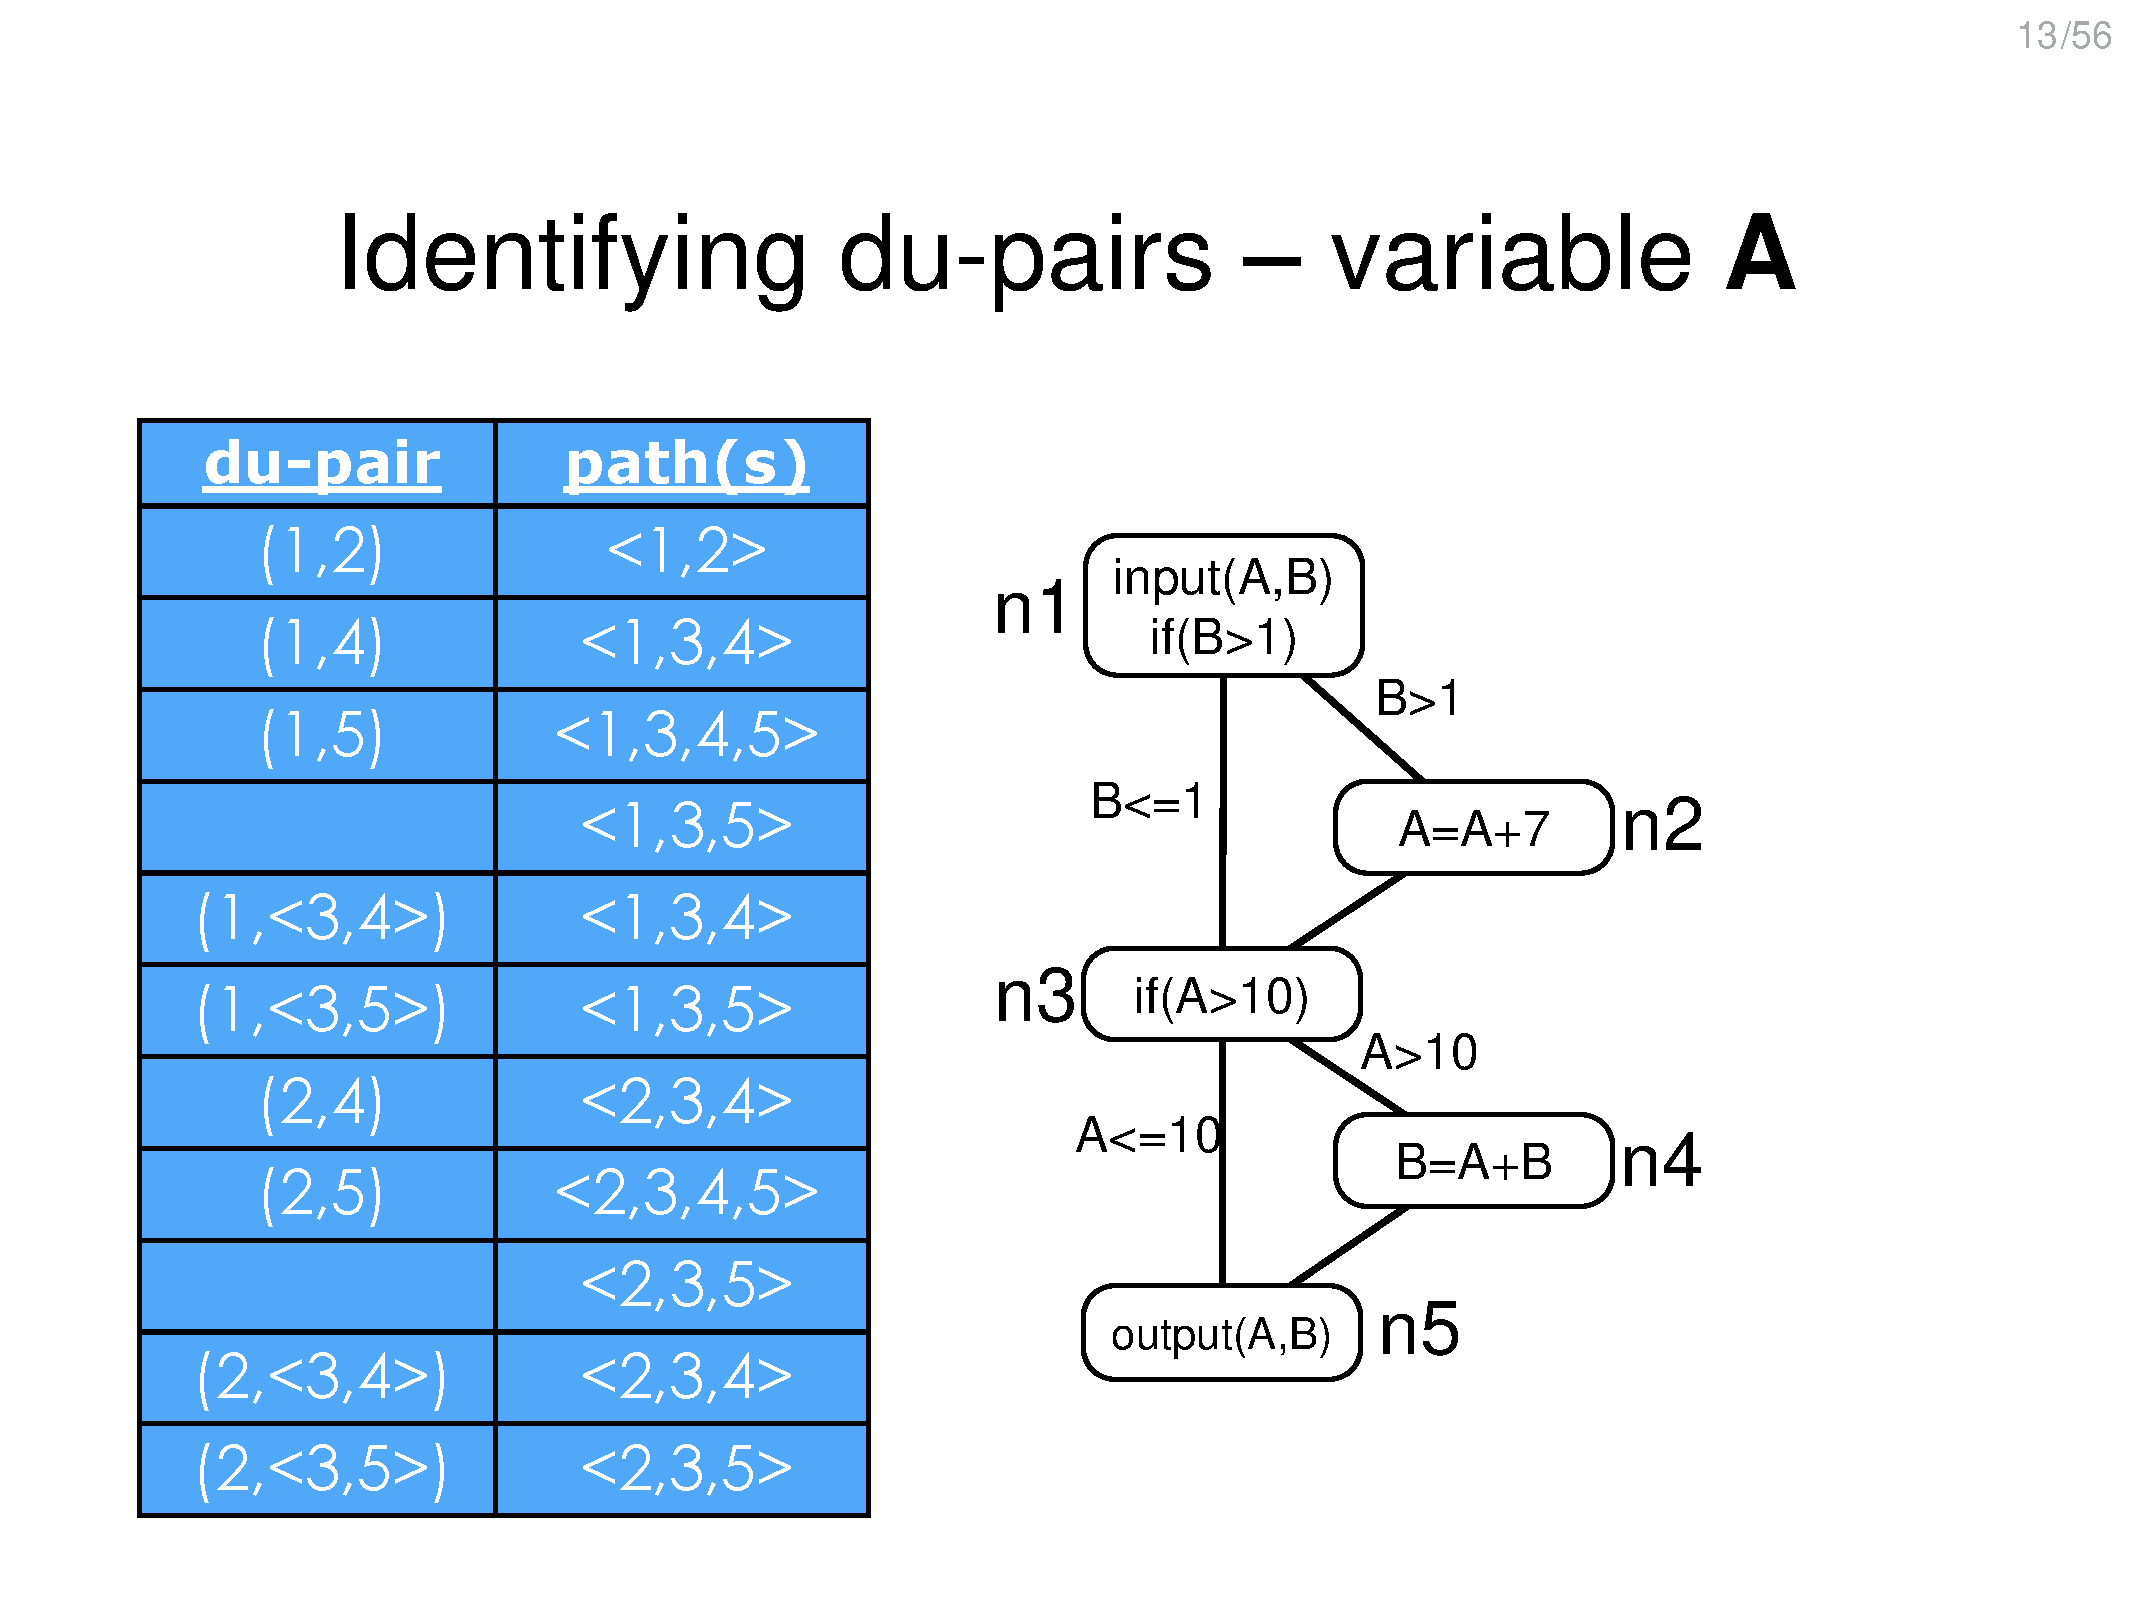
\includegraphics[width=\linewidth]{167.pdf}\\
        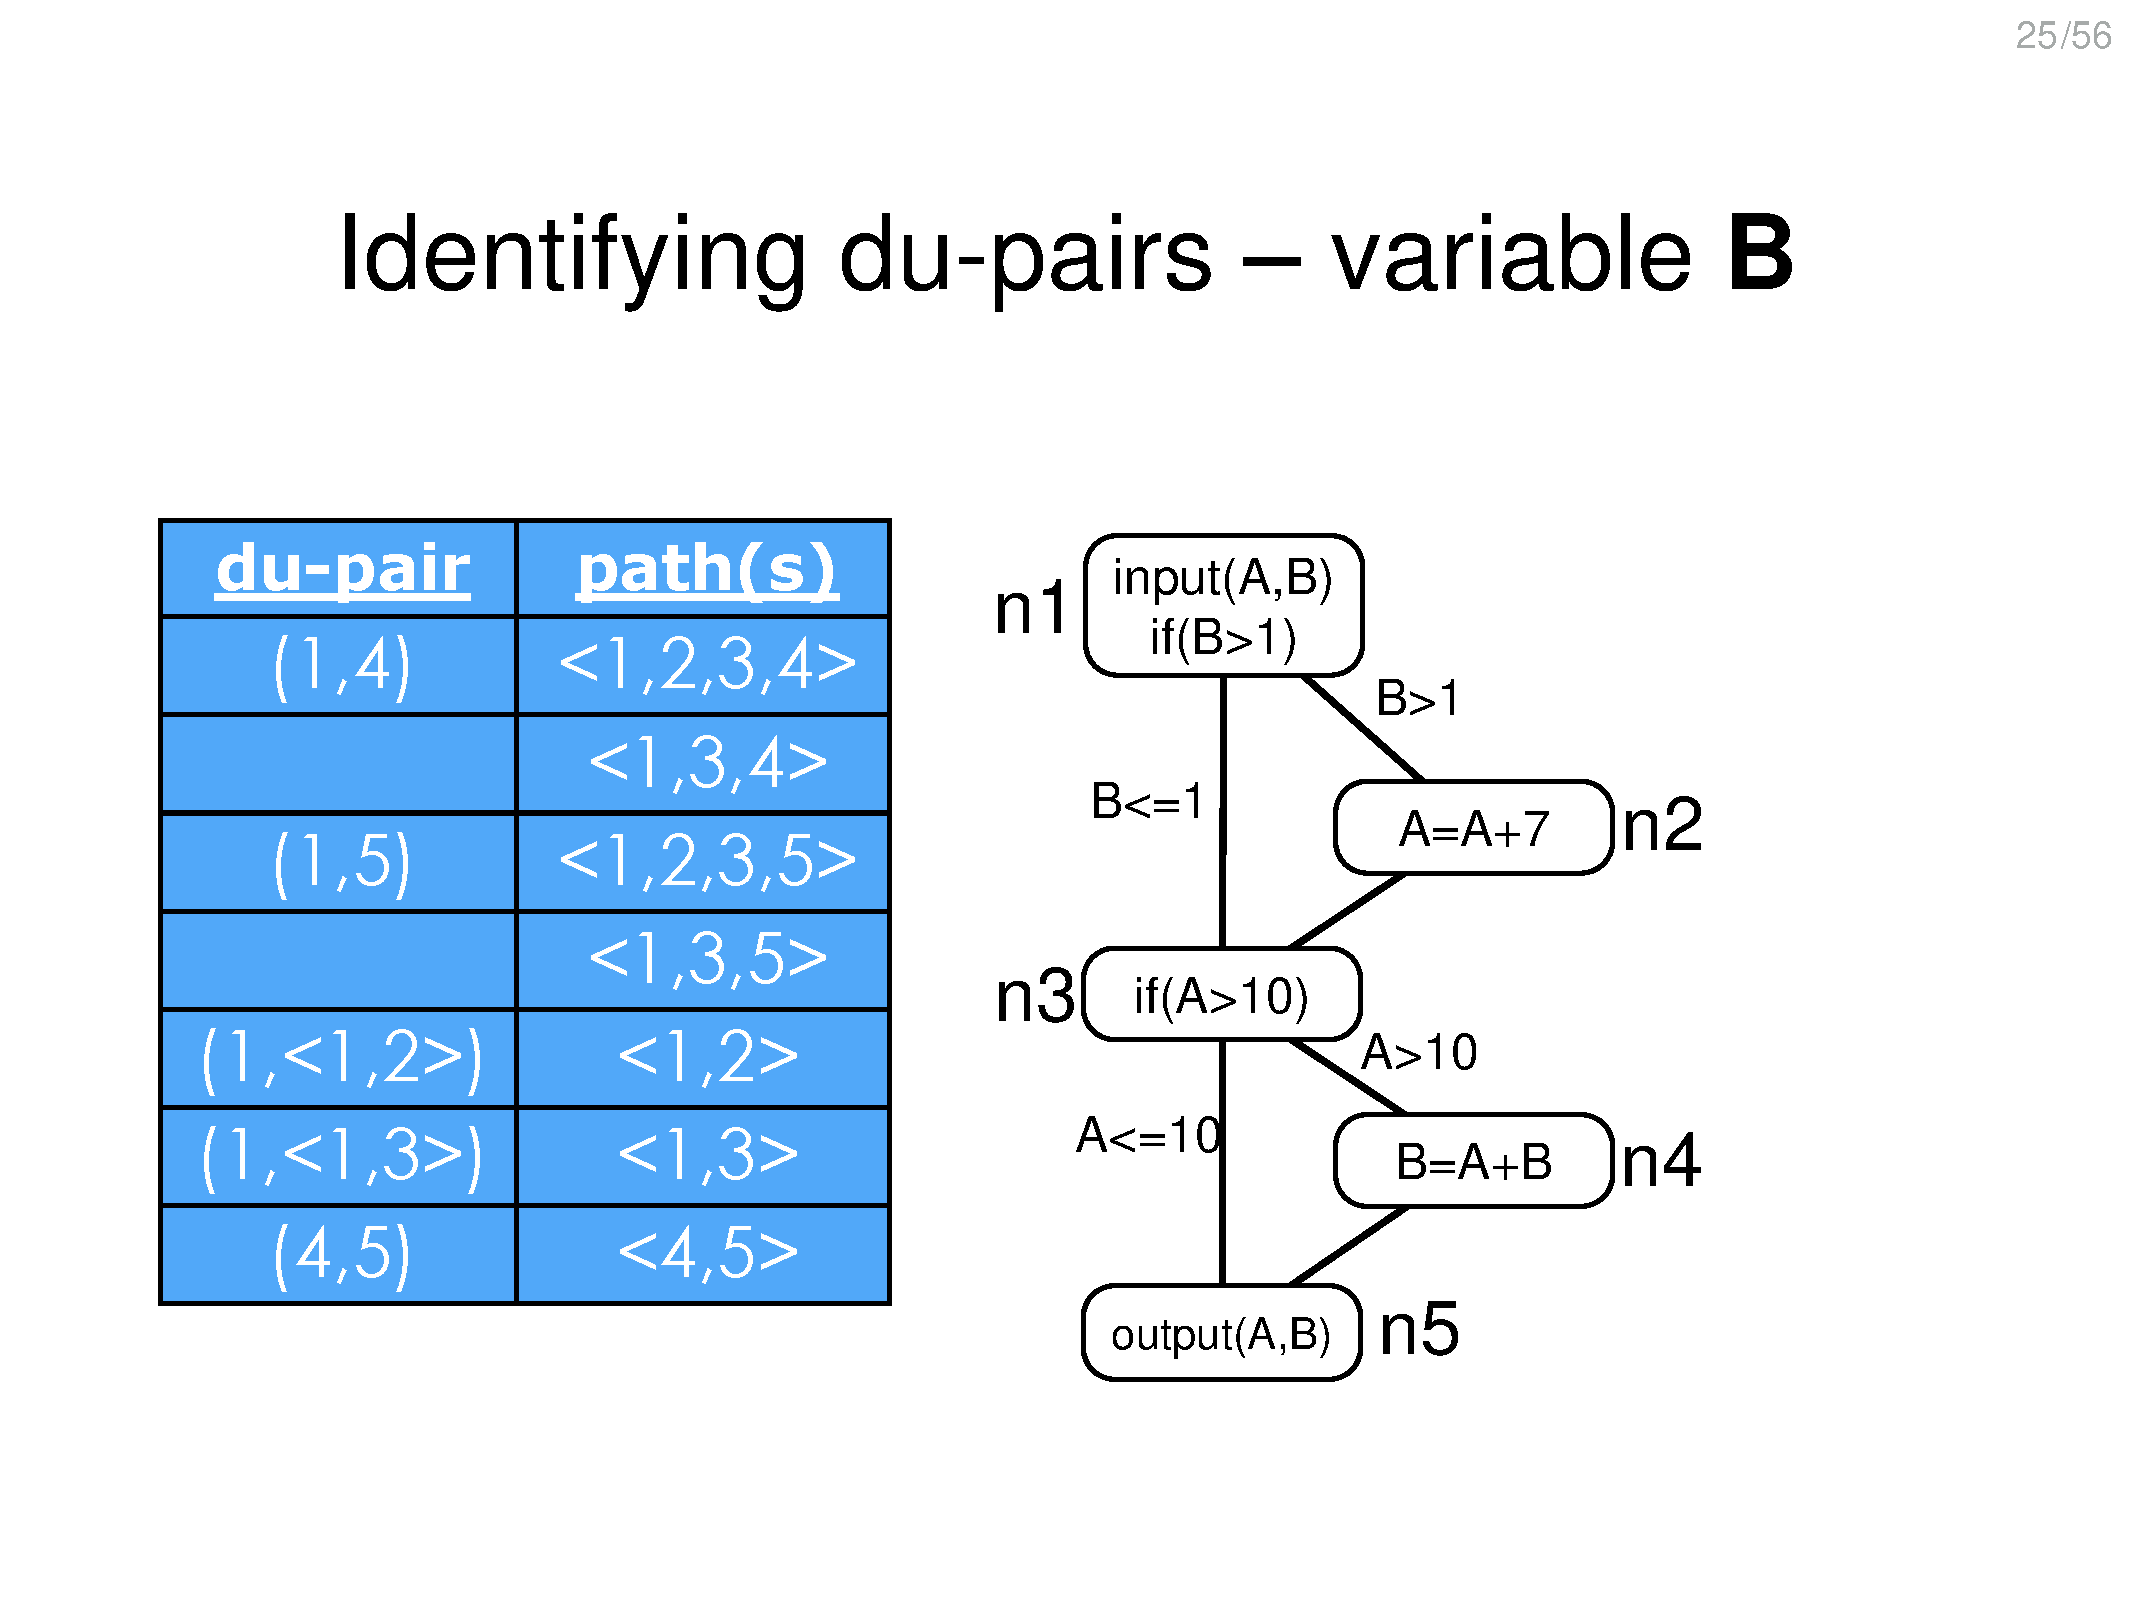
\includegraphics[width=\linewidth]{179.pdf}\\
        \textbf{\textbf{Dataflow test coverage criteria}}:\\
        \textit{All-Defs}: for every variable $v$, at least one def-clear path from every definition of $v$ to at least one c-use or p-use of $v$ must be covered\\
        \textit{All-P/C-Uses}: for every variable $v$, at least one def-clear path from every definition of $v$ to every p/c-use of $v$ must be covered\\
        \textit{All-Uses}: all du-pairs covered\\
        \textbf{Notations}:\\
        $d_1(x)$: definition of variable $x$ in node $i$\\
        $u_i(x)$: use of variable $x$ in node $i$
        $dcu(d_i(x)) = dcu(x,i)$: set of c-uses with respect to $d_1(x)$\\
        $dpu(d_i(x)) = dpu(x,i)$: set of p-uses with respect to $d_1(x)$\\
        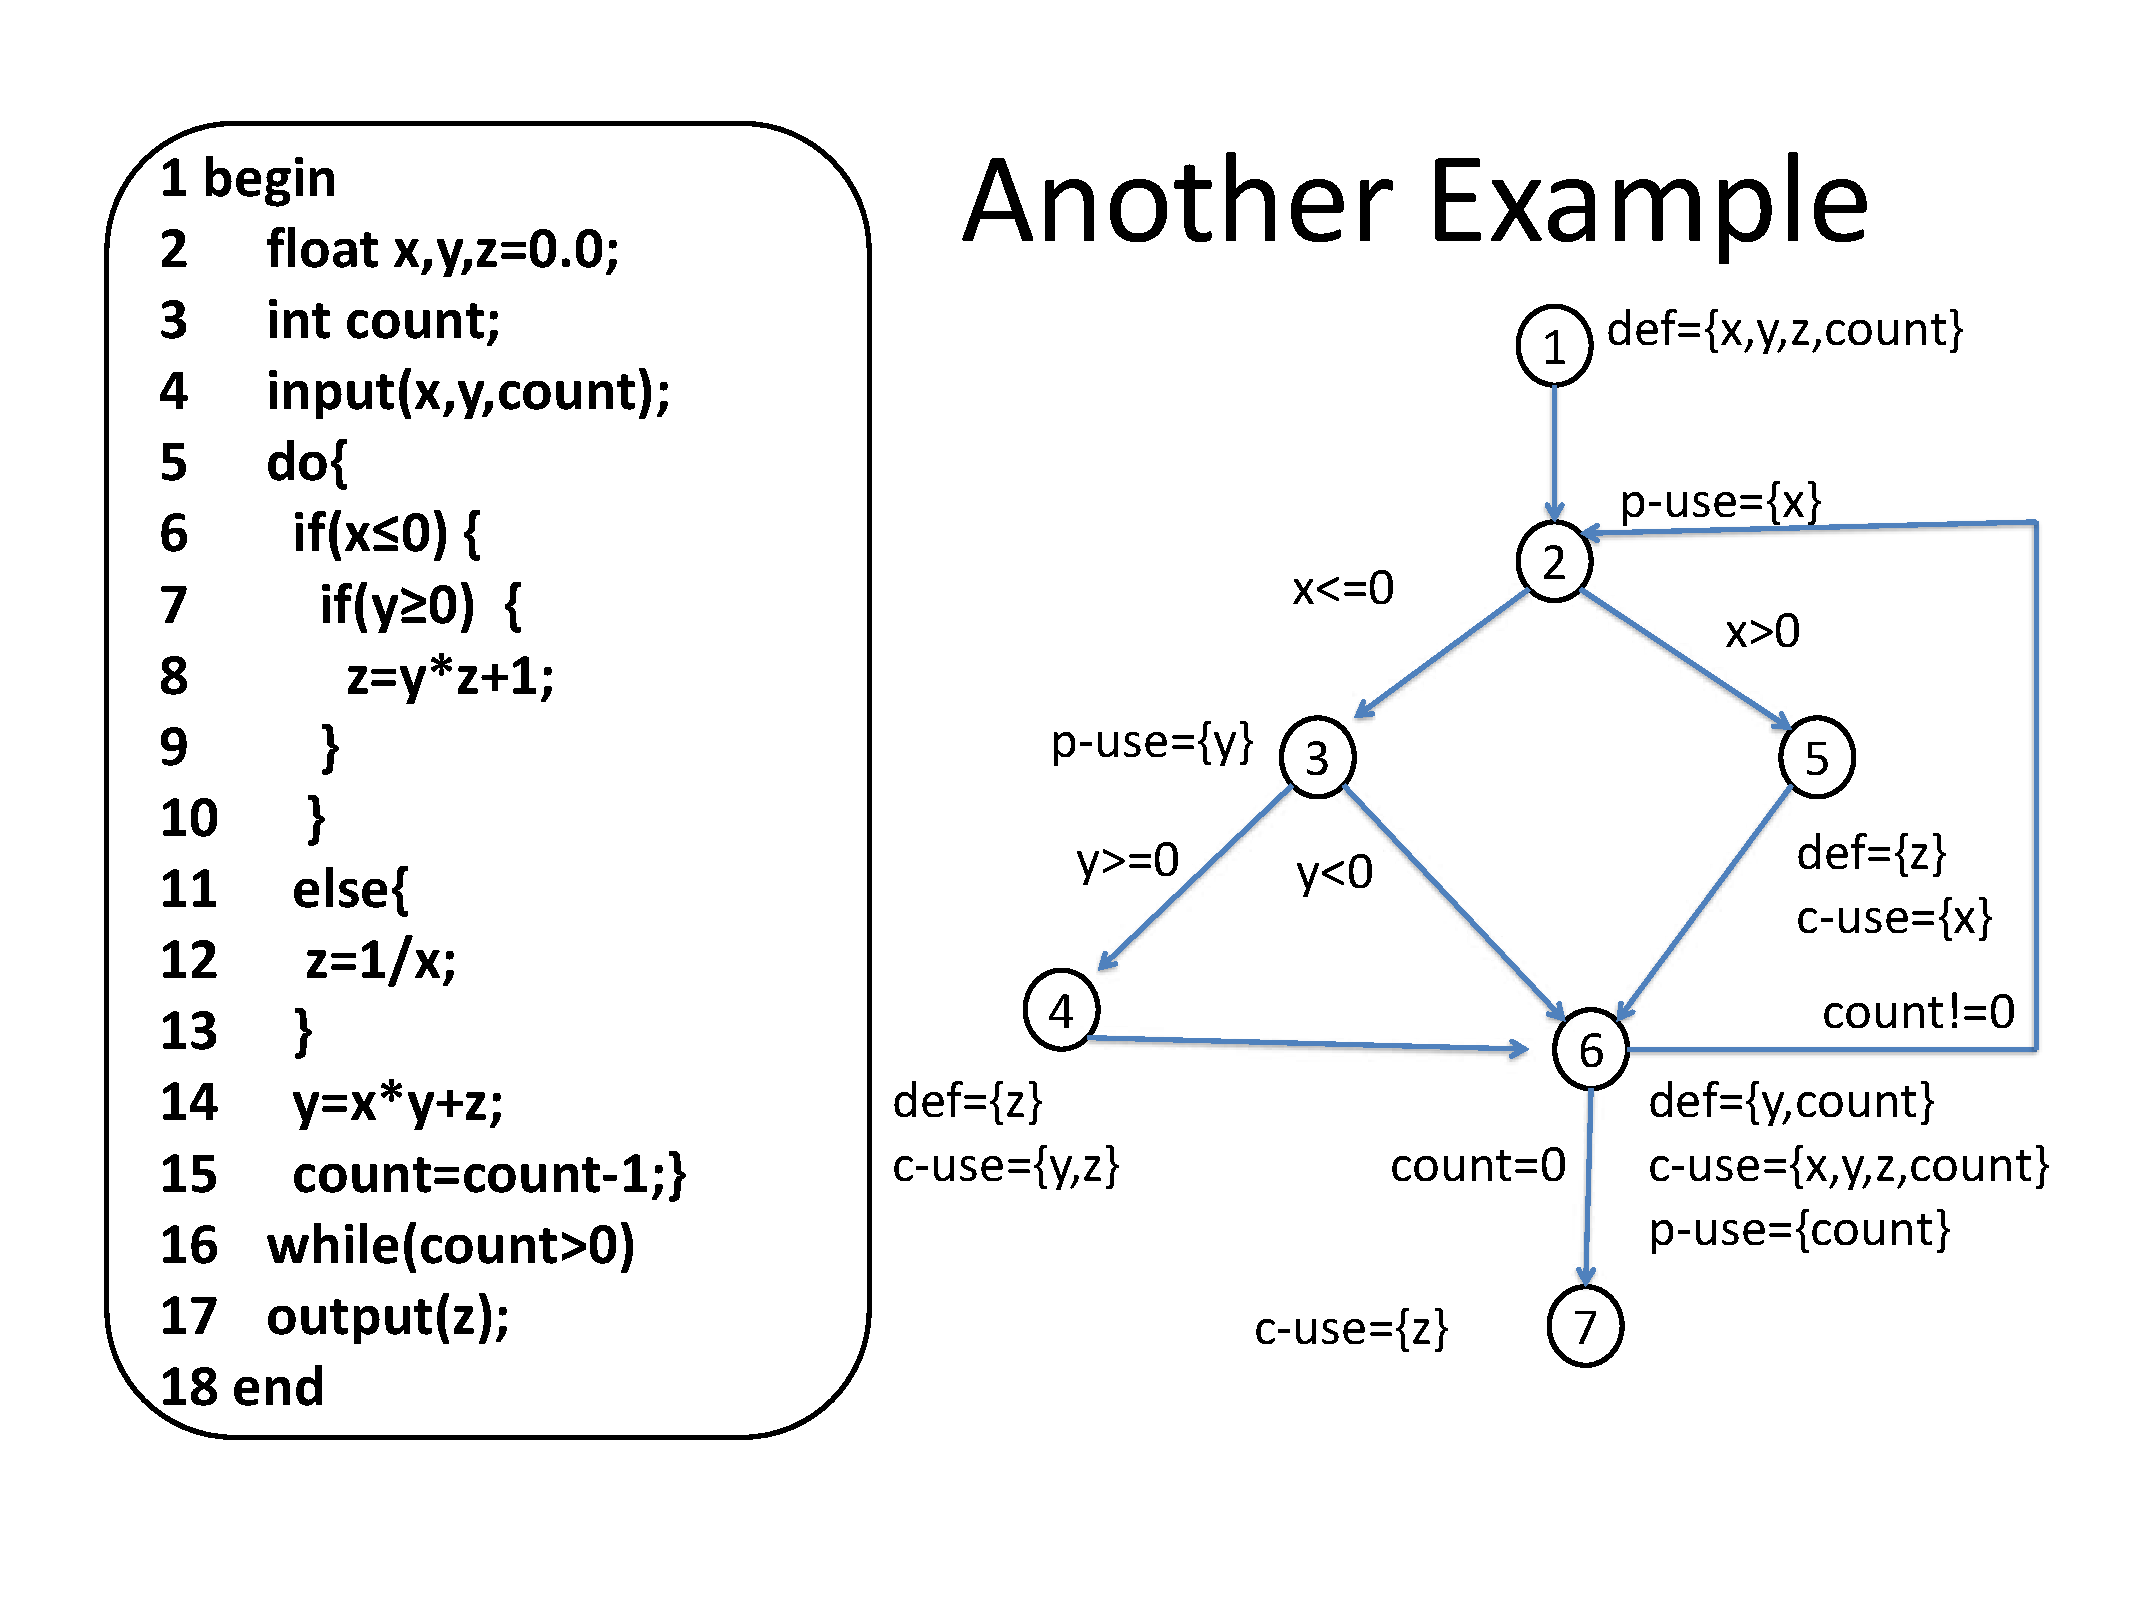
\includegraphics[width=\linewidth]{196.pdf}\\
        \textbf{All-C-Uses for above}: $dcu(x,1) + dcu(y,1) + dcu(y,6) + dcu(z,1) + dcu(z,4) + dcu(z,5) + dcu(count,1) + dcu(count,6) = 2 + 2 + 2 + 3 + 3 + 3 + 1 + 1 = 17$\\
        \textbf{All-P-Uses for above}: $dpu(x,1) + dpu(y,1) + dpu(y,6) + dpu(z,1) + dpu(z,4) + dpu(z,5) + dpu(count,1) + dpu(count,6) = 2 + 2 + 2 + 0 + 0 + 0 + 2 + 2 = 10$ (note this includes using the initial count definition even though it will always be redefined (-1) before the comparison)\\
        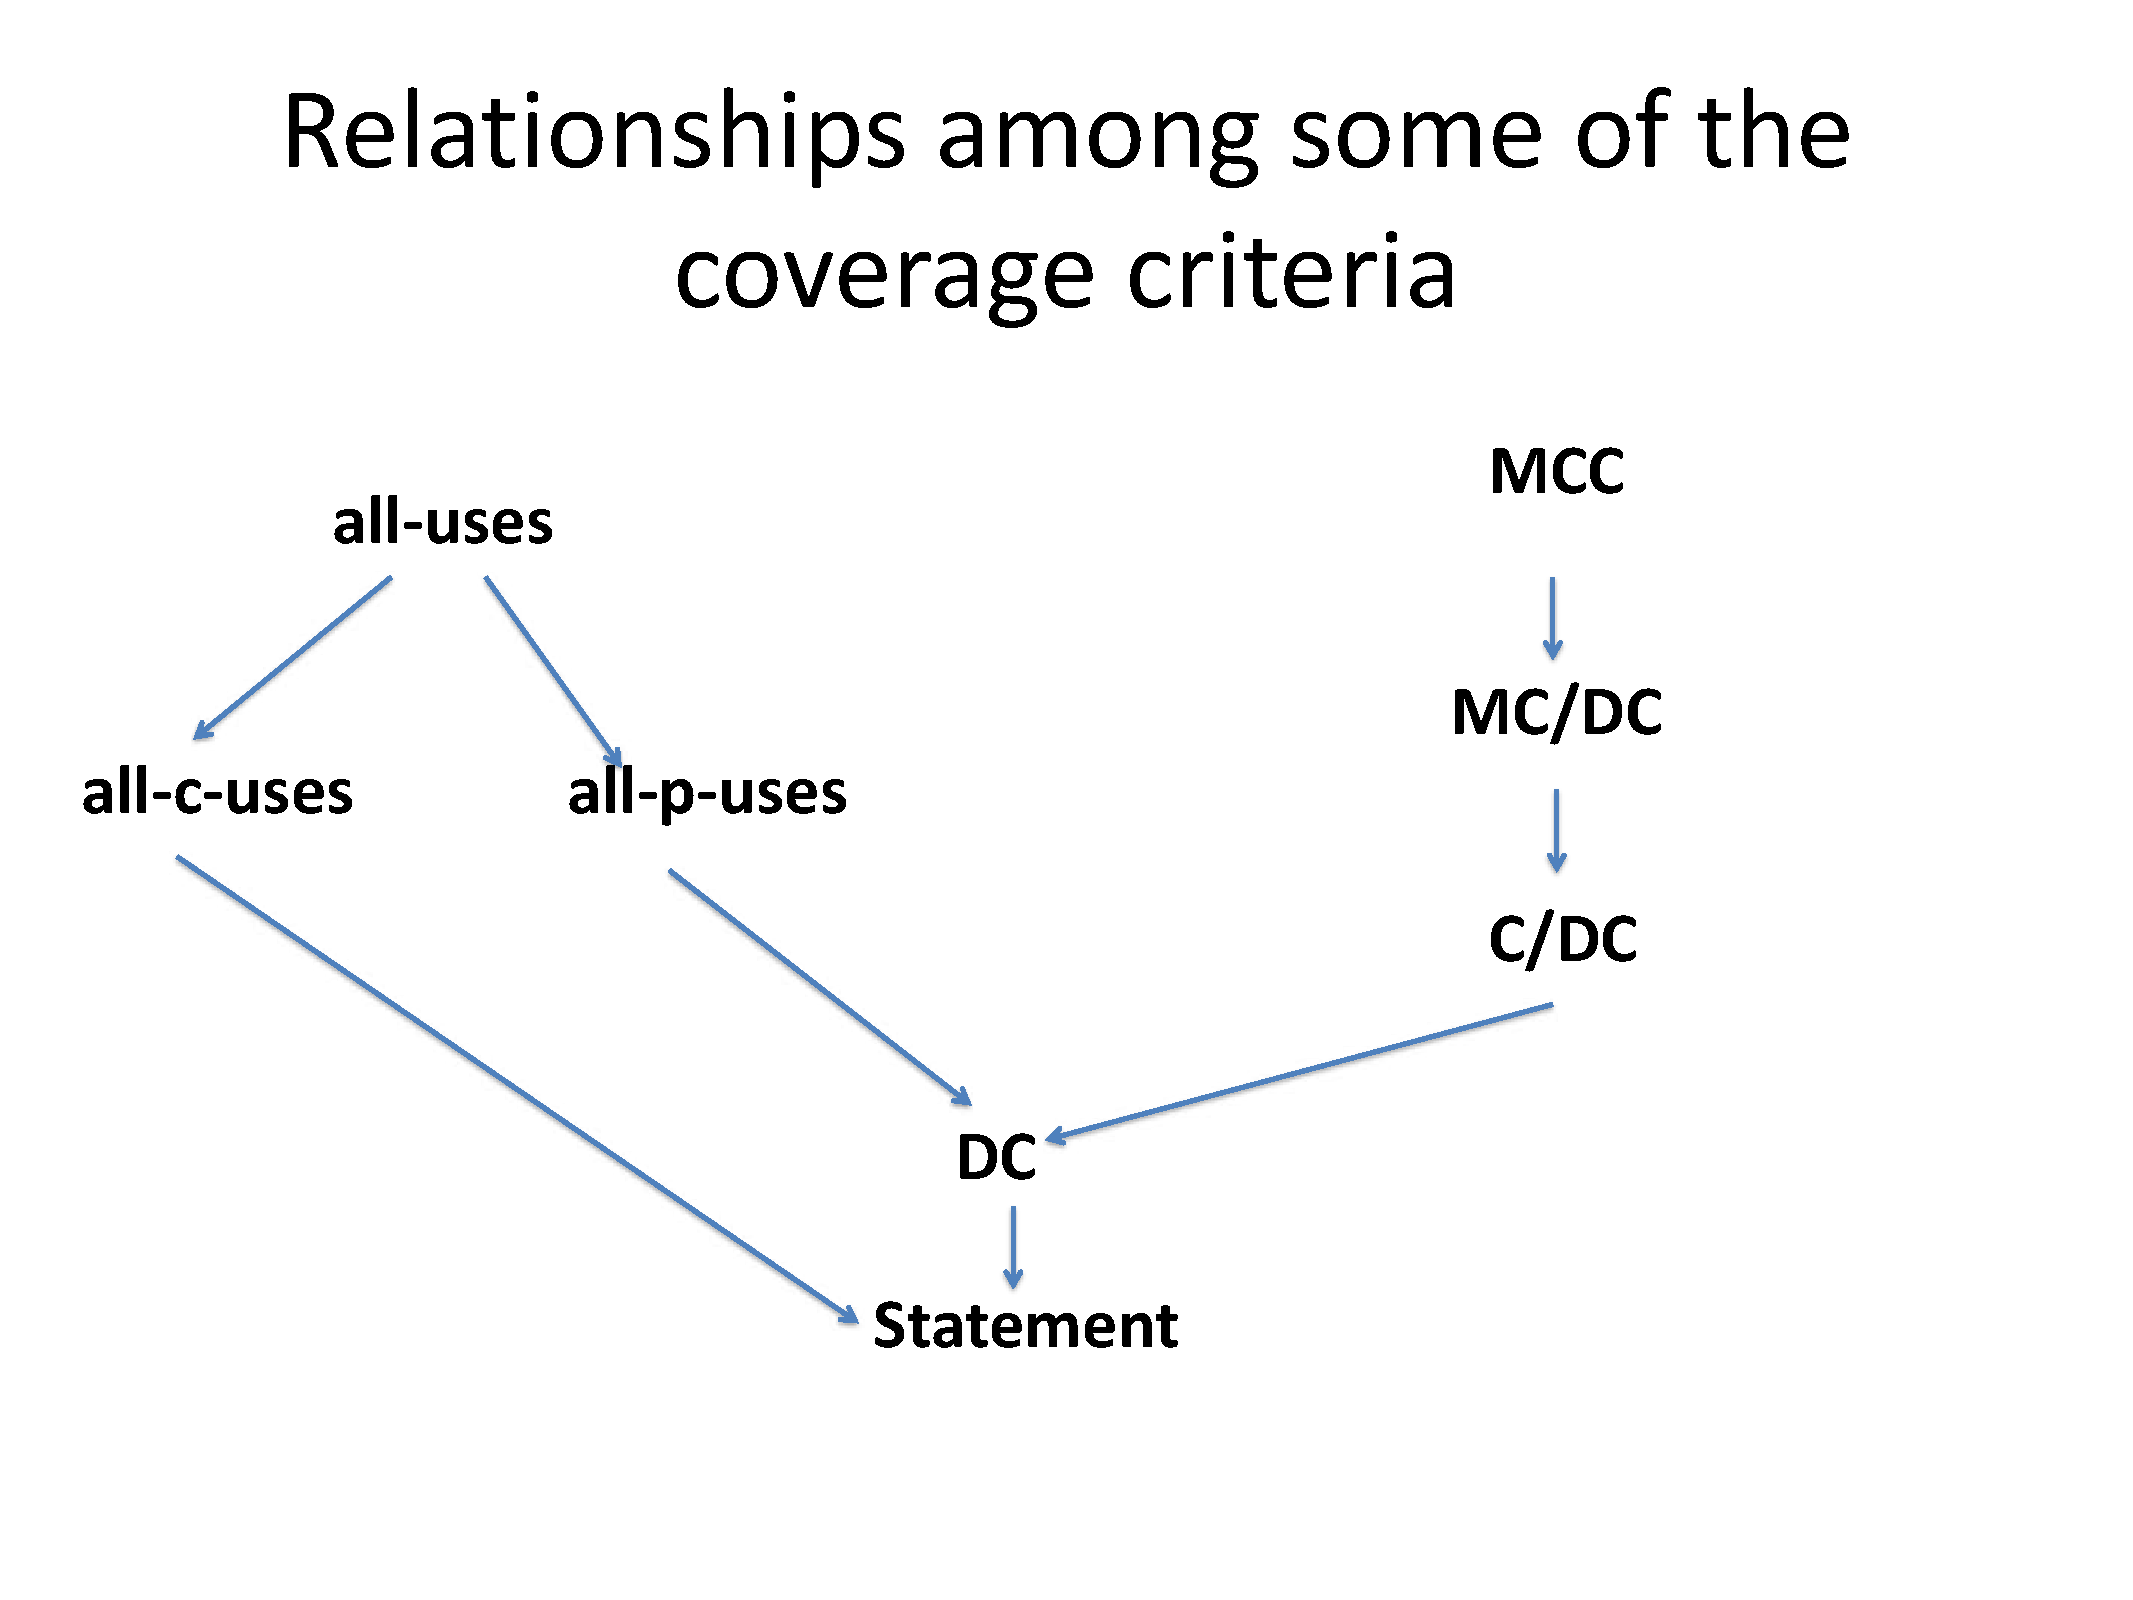
\includegraphics[width=\linewidth]{203.pdf}\\
        \underline{\textbf{Week 5}}\\
        \textbf{Program mutation}: create artificial bugs by injecting changes to statements of programs, simulate subtle bugs in real programs\\
        \textbf{Mutation testing}: software testing technique based on program mutation, can be used to evaluate test effectiveness \& enhance test suite, can be stronger than control/data-flow coverage, extremely costly since need to run whole test suite against each mutant\\
        \textbf{Mutation testing steps}: applies artificial changes based on mutation operators to generate mutants (each mutant with ony one artificial bug), run test suite against each mutant (if any test fails mutant killed, else survives), compute mutation score\\
        \textbf{Symbolic execution/evaluation}: analyse program to determine what inputs cause each part of program to execute, execute programs with symbols (track symbolic state rather than concrete input, when execute one path actually simulate many test inputs (since considering all inputs that can exercise same path))
        \textbf{Problems with symbolic execution}:\\
        \textit{Path explosion}: $2^n$ paths for $n$ branches, infinite paths for unbounded loops, calculate constraints for all paths is infeasible for real software\\
        \textit{Constraint too complex}: especially for large programs, also it is NP-complete\\
        \textbf{Input sub-domain}: set of inputs satisfying path condition\\
        \textbf{Searching input to execute path}: equivalent to solving associated path condition\\
        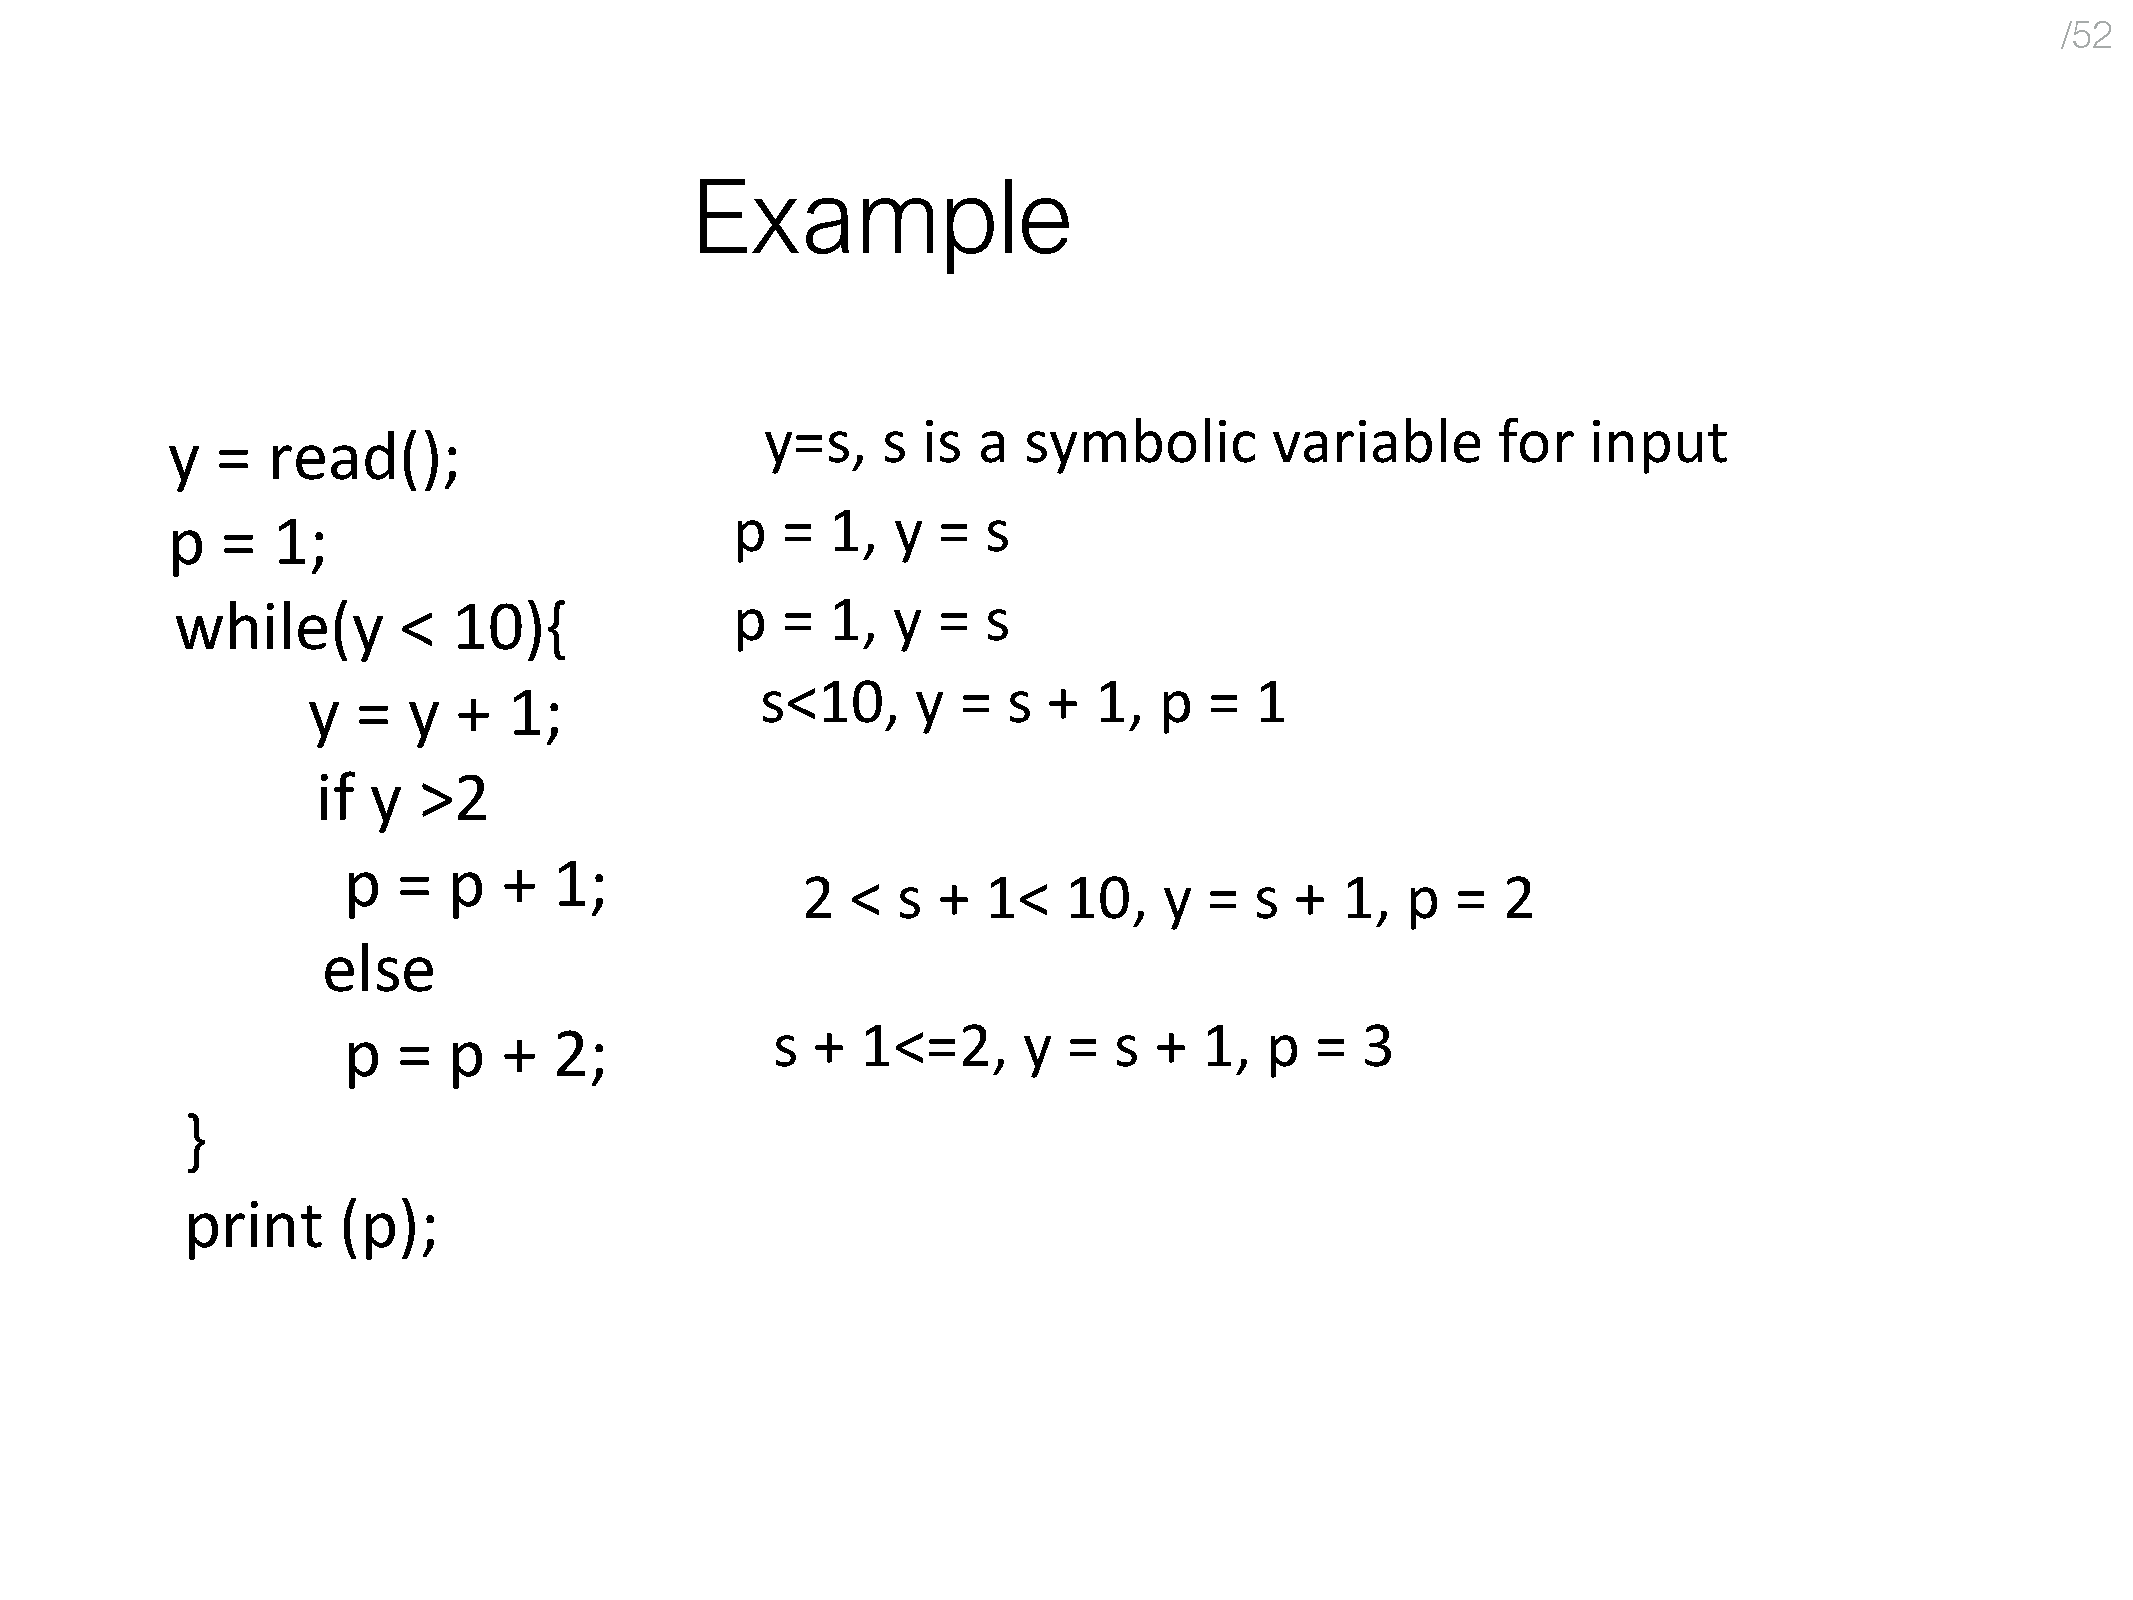
\includegraphics[width=\linewidth]{242.pdf}\\
    \end{multicols}
    \end{document}
